This section discusses the findings of the qualitative assessment. To address the formulated research questions, we perform three different experiments. Section \ref{sec:EXP1} discusses the \CT results by variating different parameters. % We measure the predict performances of the \MNB in Section \ref{sec:EXP2}. 
Finally, Section \ref{sec:EXP3} investigates the results obtained with the entangled approach \ie the combination of the two previous approaches. 


\subsection{\CT evaluation} \label{sec:EXP1}
 \rqfirst
To find the best configuration in terms of prediction performances, we experiment with different \CT configuration by variating the available parameters \ie number of neighbors \emph{k}, the recommended topic cut-off value \emph{N}, and the topic frequency cut-off \emph{t}.   %The former refers to the number of similar repositories used in the recommendation engine. 
%The latter value \emph{t} is used to select the input topics based on their frequencies: given an initial set of topics, we filter them with the cut-off value to reduce the noise in the original dataset. Then, the recommendation phase is enabled by varying the number of presented parameters. According to Section \ref{sec:methodology-metric}, N is the cut-off value and \emph{k} is the number of neighbours of the graph. We evaluate different configuration by setting N=1,5,10,15,20 and k=5,10,15,20,25. 
%Figure \ref{fig:configs} shows the results  in terms of precision and recall. 


As we are relying on a collaborative filtering technique, the number of output topics, the number of neighbours, and the data preprocessing play an important role in the assessment. Thus, we variate  the recommended list of topics \emph{N} for 5 and 10, and the number of neighbours \emph{k} \ie \emph{N} = \{5, 10, 15, 20, 25\}. Moreover, we use different topic frequency cut-off \emph{t} to remove very infrequent topics from the dataset. 
The bar charts in Fig.~\ref{fig:success-rateN5} and \ref{fig:success-rateN10} show the average success rates of all ten folds of \CT, divided by the different topic frequency cut-off \emph{t}. In particular, Fig.~\ref{fig:success-rateN5} and Fig.~\ref{fig:success-rateN10} shows the success rate considering the first 5 and 10 recommended topics respectively. The horizontal axes shows the success rate outcomes for different size of neighbours \emph{N}.
Overall, it is evident that infrequent topics negatively affect both success rate values. At the first glance we can see that the success rate of \CT with all topics is much lower than others \emph{t} cut-off.
\begin{figure*}[t]
\centering
	\begin{tabular}{c c}	
	\subfigure[Success rate@5]{\label{fig:success-rateN5}
	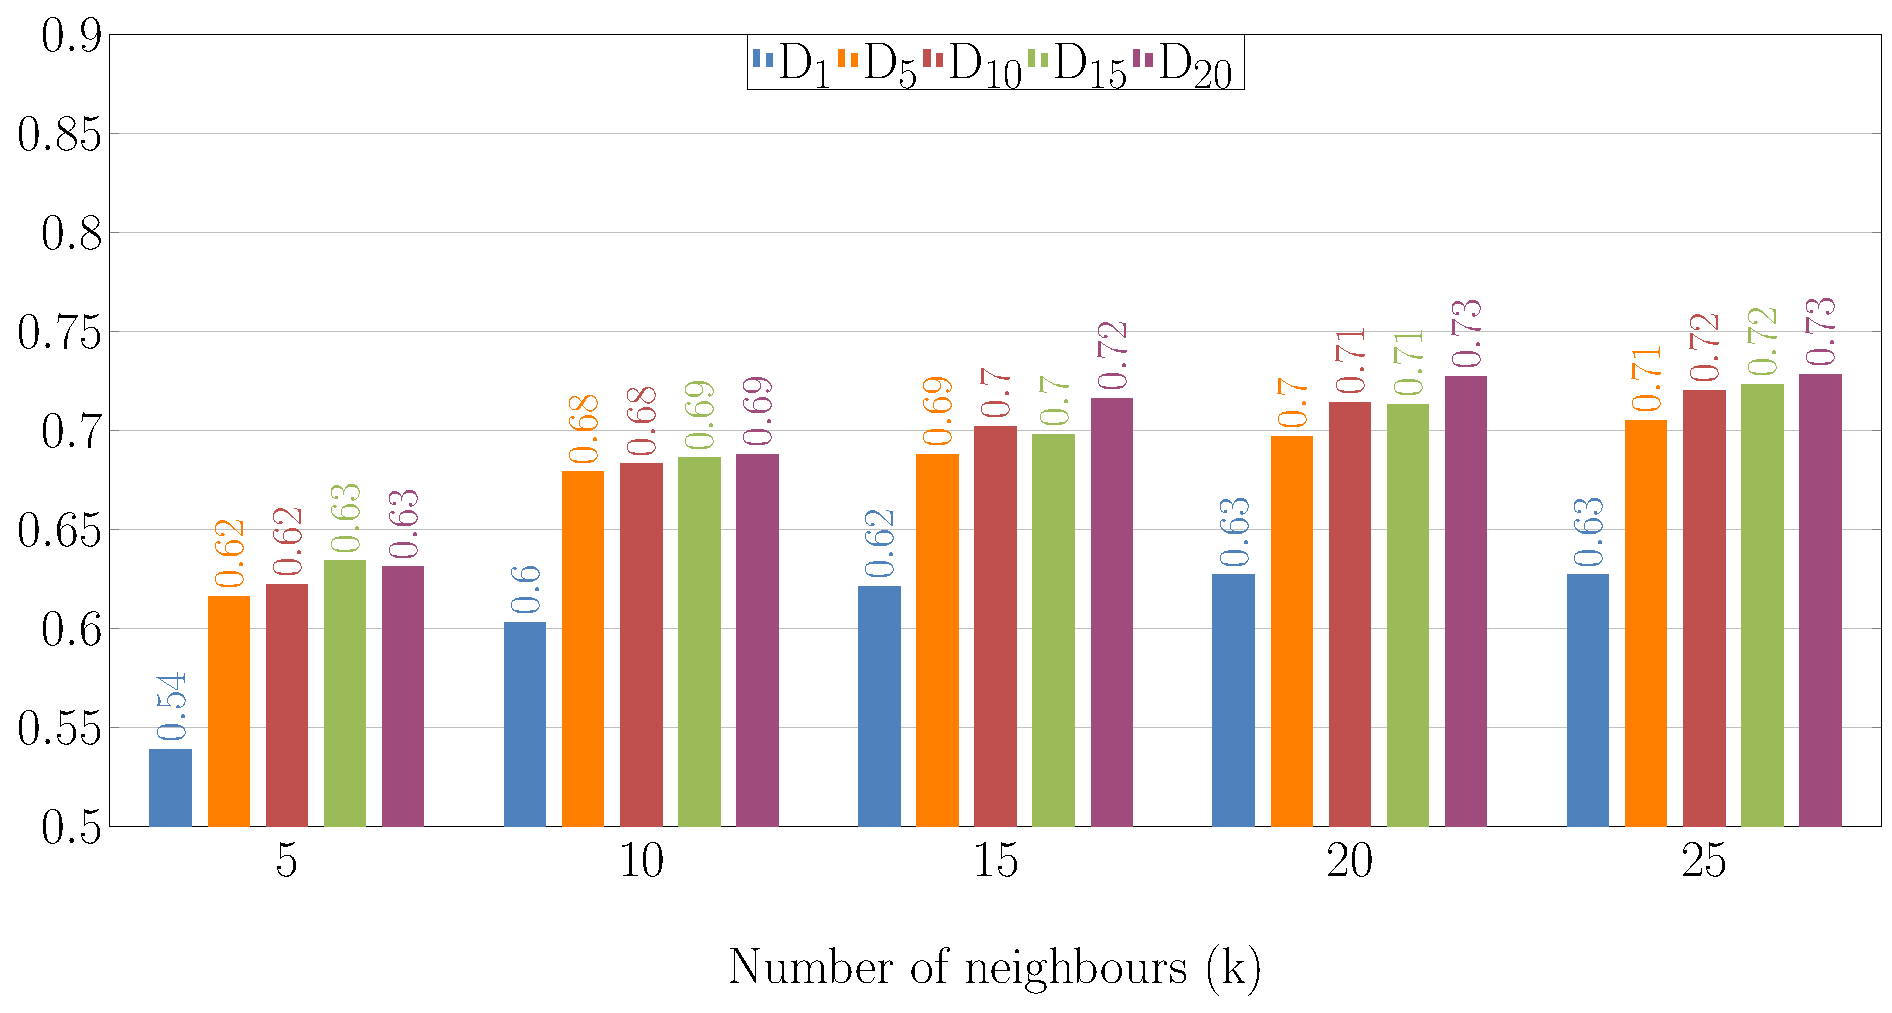
\includegraphics[width=0.45\linewidth]{figs/successRateN@5.pdf}} &
	\subfigure[Success rate@10]{\label{fig:success-rateN10}
	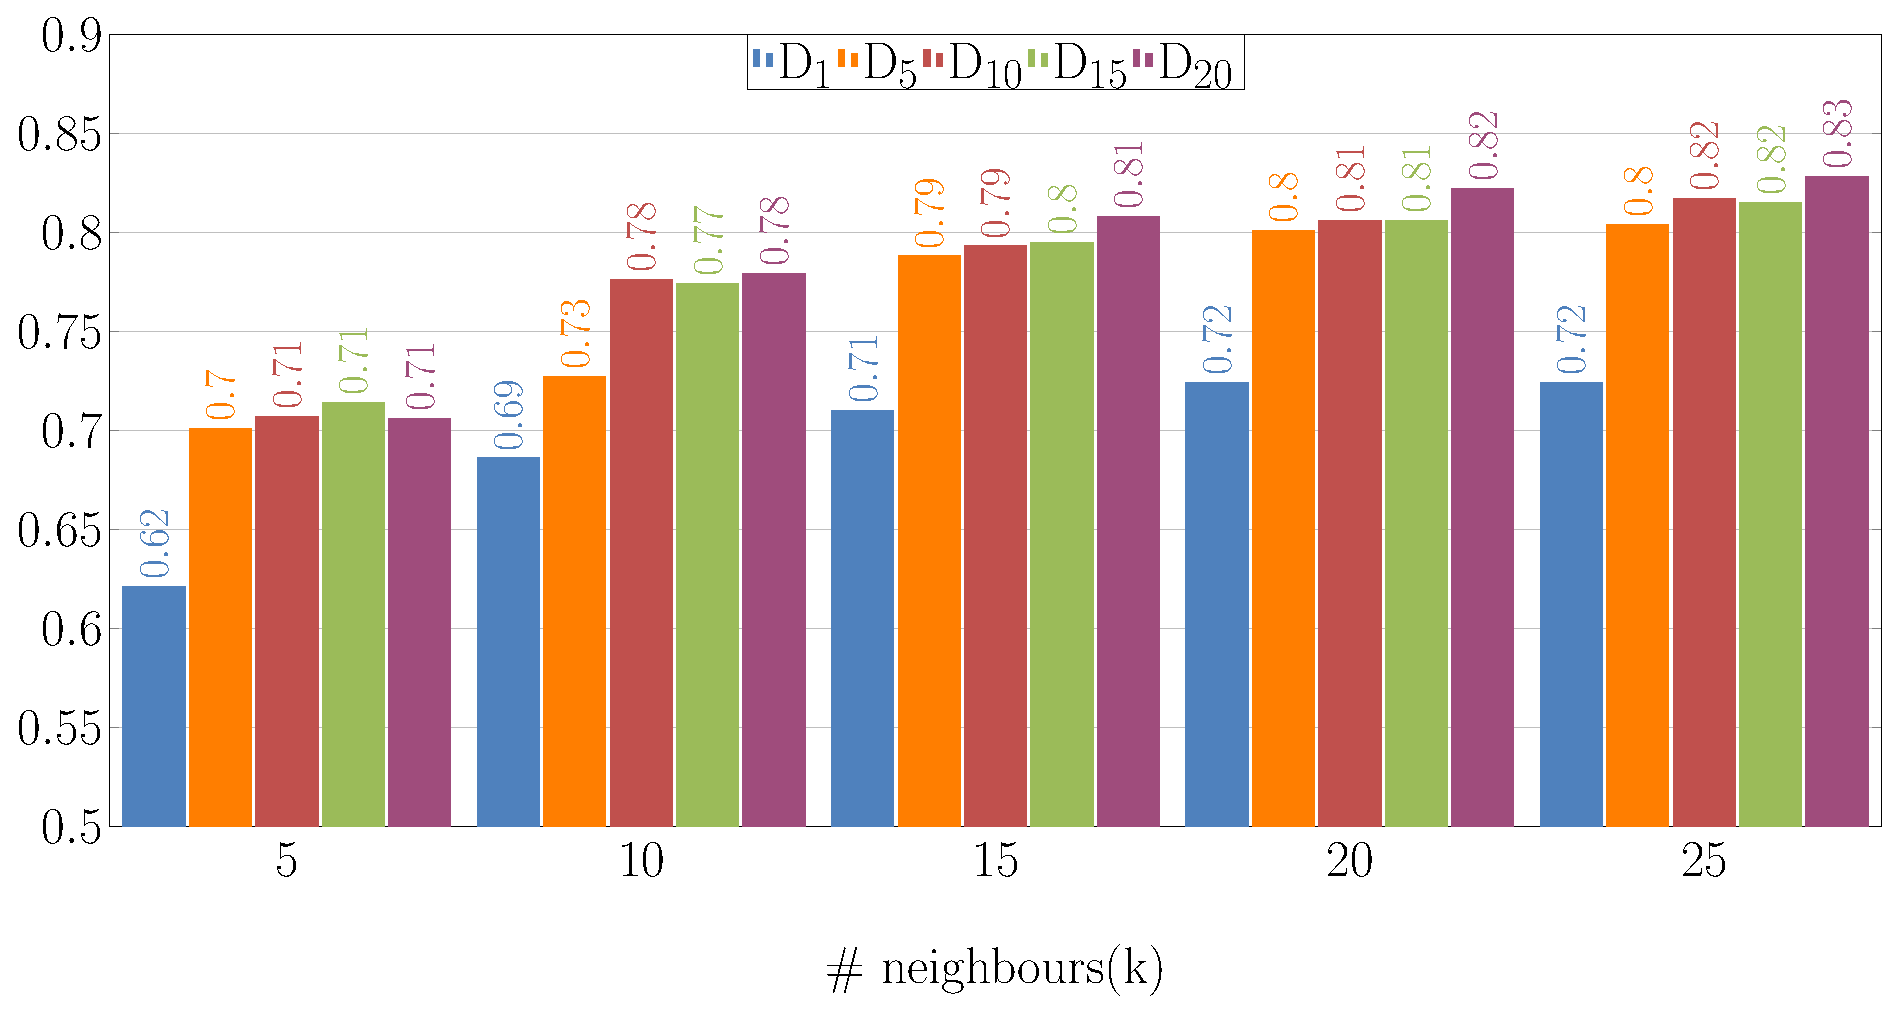
\includegraphics[width=0.45\linewidth]{figs/successRateN@10.pdf}}
	
	\end{tabular} 
	\caption{Success rate with 5 and 10 input topics.}
	\label{fig:success5_10}
\end{figure*}
\begin{figure}[t!]
	\centering
	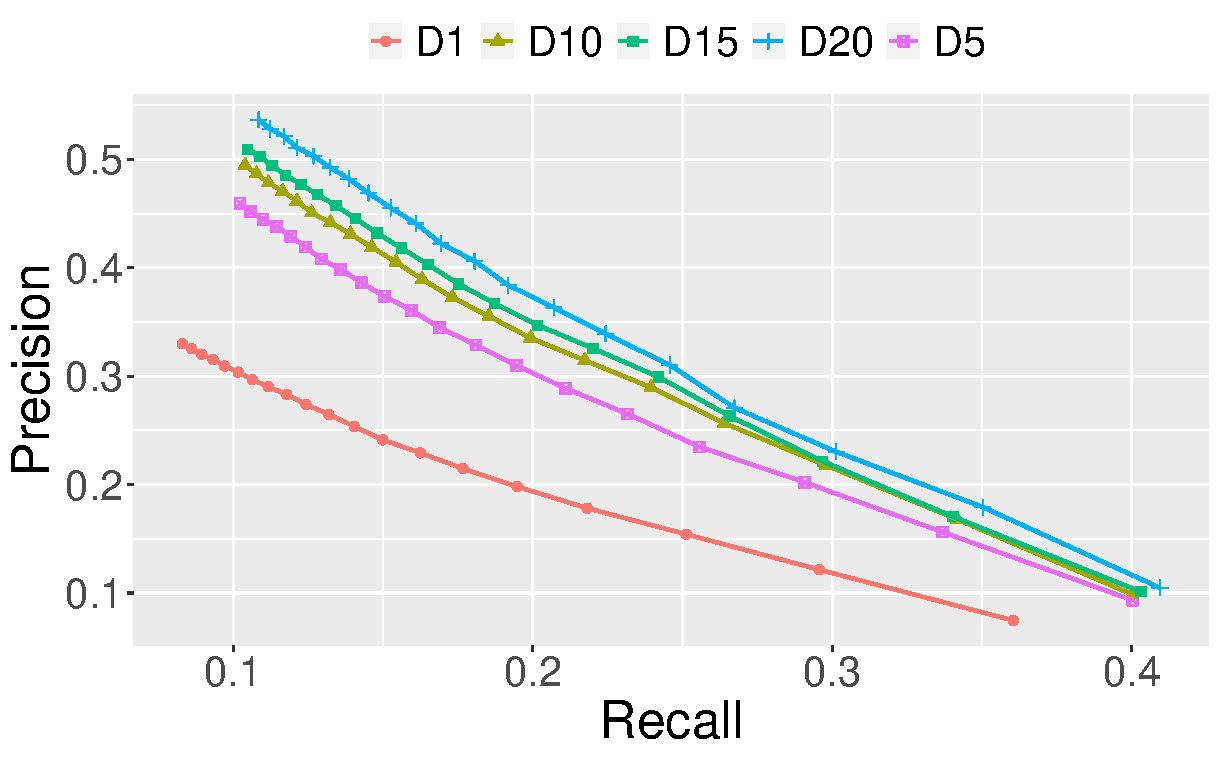
\includegraphics[width=\linewidth]{figs/PrecisionRecallCurve.pdf}
	\caption{Evaluation of the different configuration.}
	\label{fig:configs}
\end{figure}
The success rate assessment exhibits an average improvement of 10\% in all of the possible configurations obtained by variating \emph{N} and \emph{k} values. In particular, the success rate archives better results by setting higher values of \emph{k}. Nevertheless, increasing the number of neighbors gives remarkable benefits only until a certain threshold. Given \emph{k} = 5, the success rate@5 passes from 63\% to 69\% if we consider k=10. This positive delta decreases by augmenting the number of neighbours until it reaches a stable success rate. Thus, we can consider \emph{k} = 25 as the maximum value capable of improving prediction performances. This trend is further confirmed by introducing more topics in the initial set. We also demonstrate that the topic filtering preprocessing fosters this enhancement and noise removal is a critical step of the entire process.

This is also confirmed by the precision and recall curves depicted in Fig.~\ref{fig:configs}. 
%From the accuracy scores computed using Eq. (5) and Eq. (6), the Precision-Recall curves (PRCs) for all 10 rounds of validation and different values of k were sketched. 
The line graph depicts the precision and recall curves on average for all 10 rounds by considering \emph{N} value ranges from 1 to 20 and \emph{t}. So, each dot in a curve corresponds to a specific value of \emph{N}. 
These outcomes have been obtained by keeping 25 as the number of neighbours \emph{k} because we have already discussed that higher values of neighbours reach better prediction performances. Overall, the precision and recall values rise when the \emph{t} cut-off grows. Given that better prediction performance appears near to the upper right corner~\cite{DiNoia:2012:LOD:2362499.2362501}, the figure shows that a higher value of \emph{t} reaches better accuracy for all values of \emph{N}.

In the methodology described in Section~\ref{sec:methodology-metric}, for each repository \emph{r}, the evaluation outcomes consider the half part of real topics as input and remaining ones as ground truth data \emph{GT(r)}. Because of we are also interested to understand how the number of input topics impacts on prediction performance, Fig.~\ref{fig:pr-input-topics} shows the average success rate of all ten folds by choosing different number of input topics. Varying |\emph{t$_{in}$}| means changing the length of input topics that enable the \CT collaborative filtering recommender. In this picture we report the average success of all folds values for the best configuration settings (\ie \emph{k} = 25, \emph{t} = 20 and) . The success rate values exhibits an improvements when the size of input topic rises. This  behaviour demonstrate that \CT computes better similar repositories as neighbours when it has a higher number of topic as input. This is due to the similarity function that has been involved in the computation of first  \emph{k} neighbours. Because the average number of topics for each considered repository is 9.896 we can consider |\emph{t$_{in}$}| = 5 as the maximum value capable of improving prediction performances.
\begin{figure}[t!]
	\centering
	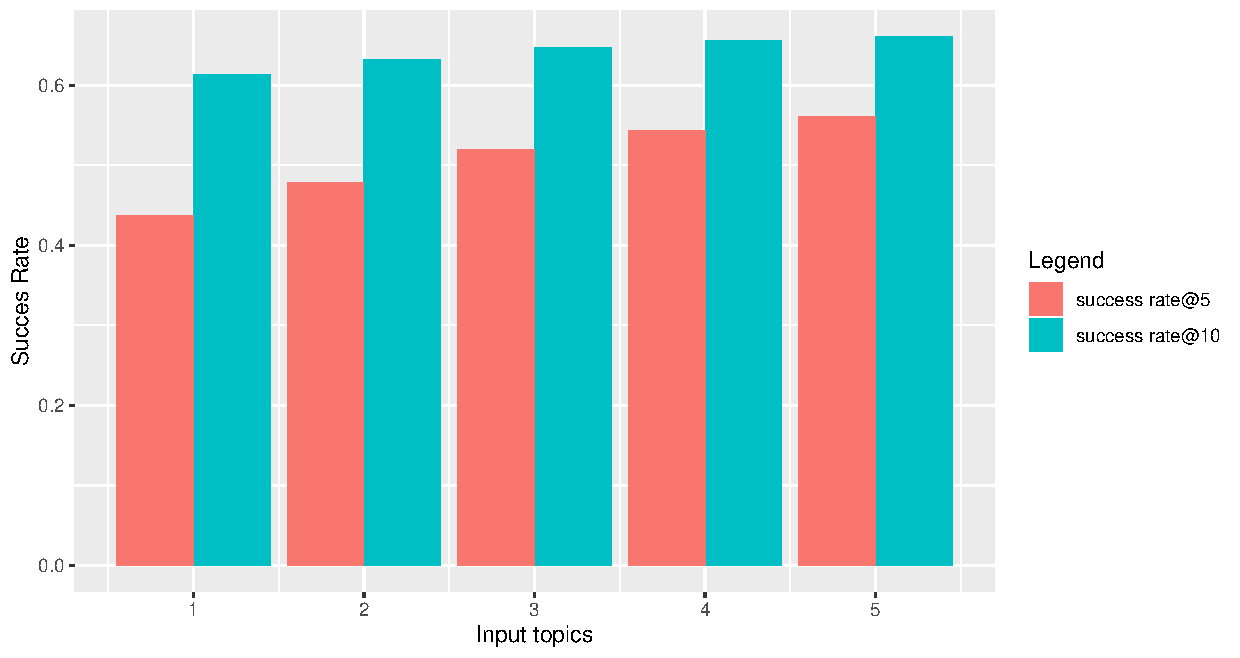
\includegraphics[width=\linewidth]{figs/sr_change_input_topics.pdf}
	\caption{Evaluation of the different input topics.}
	\label{fig:pr-input-topics}
\end{figure} 

\begin{tcolorbox}[boxrule=0.86pt,left=0.3em, right=0.3em,top=0.1em, bottom=0.05em]
The quality evaluation demonstrates that \CT achieves better results by increasing the input data. The number of neighbors and the topic filters contribute to this improvement. However, the precision and recall values are still low, suggesting that bias lives in the users topic.
\end{tcolorbox}


%\subsection{\MNB evaluation} \label{sec:EXP2}

\rqsecond

Due to the lack of a baseline, we investigate the prediction performances of the \MNB to compare its outcomes with \CT. Reversely from the original paper, we apply the \MNB and we compared the outcomes whit respect to all topics (includin non featured ones) leaving the underlying structure untouched. This is necessary to undertake a fair comparison with \CT. Table \ref{tab:compareMNB} shows the evaluation results in terms  of the three aforementioned metrics. 


%\begin{table}[h]
%\centering
%
%
%\resizebox{8.5cm}{!} {
%\begin{tabular}{|l|l|l|l|l|l|l|}
%\hline
%  & \multicolumn{3}{c|}{ \textbf{\MNB}}          & \multicolumn{3}{c|}{ \textbf{\CT}}        \\ \hline
%\textbf{No. of input} & \textbf{Success rate} &\textbf{ Precision} & \textbf{Recall} & \textbf{Success rate} &\textbf{ Precision} &\textbf{ Recall} \\ \hline
%2  &       0.220       &    0.117       &  0.031       &     0.554         &      0.350     &   0.179      \\ \hline
% 4 &     0.392         &    0.119       &     0.063   &       0.682       &       0.267    &   0.271     \\ \hline
%6 &    0.538          &      0.122	     &   0.096     &     0.754         &    0.224       &   0.339     \\ \hline
%8 &    0.648          &  0.119         &   0.125      &         0.803     &     0.192      &   0.384     \\ \hline
%10 &      0.711        &    0.112       &   0.147     &      0.828        &   0.169        &    0.422    \\ \hline
%12 &     0.765         &      0.112     &   0.177     &        0.851      &     0.153      &     0.455   \\ \hline
%14 &      0.815        &    0.119       &   0.220     &    0.863          &   0.139         &   0.482     \\ \hline
%16 &       0.853       &     0.112      &     0.258   &        0.879      &   0.127        &   0.503     \\ \hline
%18 &      0.874        &     0.122      &     0.290   &       0.886       &     0.117      &    0.521    \\ \hline
%20 &     0.891         &    0.121       &    0.320    &      0.892        &   0.117        &       0.537 \\ \hline
%\rowcolor{Gray}
%\textbf{Average values} &    \textbf{0.651}        &   \textbf{ 0.120}       &   \textbf{ 0.165 }  &     \textbf{ 0.785}        &  \textbf{ 0.194}        &     \textbf{ 0.397 } \\ \hline
%\end{tabular}
%}
%\caption{Comparison of the two approaches.}
%\label{tab:compareMNB}
%\end{table} 
% Please add the following required packages to your document preamble:
% \usepackage[table,xcdraw]{xcolor}
% If you use beamer only pass "xcolor=table" option, i.e. \documentclass[xcolor=table]{beamer}
\begin{table}[]
	\scriptsize
	\resizebox{8.5cm}{!} {
	\begin{tabular}{|l|l|l|l|l|l|l|}
		\hline
		\rowcolor[HTML]{C0C0C0} 
		& \multicolumn{2}{c}{\textbf{Success rate}}         & \multicolumn{2}{|c|}{\textbf{Precision}}            & \multicolumn{2}{c|}{\textbf{Recall}}               \\ \hline
	 \rowcolor[HTML]{C0C0C0} 
		\textbf{\emph{N} } & \textbf{MNB} & \textbf{\CT }& \textbf{MNB} & \textbf{\CT} & \textbf{MNB} & \textbf{\CT }\\ \hline
		2                       & 0.220               & 0.554              & 0.117               & 0.350              & 0.031               & 0.179              \\
		4                       & 0.392               & 0.682              & 0.119               & 0.267              & 0.063               & 0.271              \\
		6                       & 0.538               & 0.754              & 0.122               & 0.224              & 0.096               & 0.339              \\
		8                       & 0.648               & 0.803              & 0.119               & 0.192              & 0.125               & 0.384              \\
		10                      & 0.711               & 0.828              & 0.112               & 0.169              & 0.147               & 0.422              \\
		12                      & 0.765               & 0.851              & 0.112               & 0.153              & 0.177               & 0.455              \\
		14                      & 0.815               & 0.863              & 0.119               & 0.139              & 0.220               & 0.482              \\
		16                      & 0.853               & 0.879              & 0.112               & 0.127              & 0.258               & 0.503              \\
		18                      & 0.874               & 0.886              & 0.122               & 0.117              & 0.290               & 0.521              \\
		20                      & 0.891               & 0.892              & 0.121               & 0.117              & 0.320               & 0.537              \\ \hline
		\rowcolor[HTML]{C0C0C0} 
		\textbf{Average} & \textbf{0.651}      & \textbf{0.785}     & \textbf{0.120}      & \textbf{0.194}     & \textbf{0.165}      & \textbf{0.397}    \\ \hline
	\end{tabular}}
\caption{Comparison of the two approaches.}
\label{tab:compareMNB}
\end{table}
We evaluate both approaches by variating the number of recommended topics up to 20. For the sake of the presentation, we report half of the data as we aim to show the overall trend.
As we can see, \CT outperforms the \MNB considering all the metrics. In particular, the success rate grows according to the number of input for both of the approaches. Although the \MNB reaches the same values of \CT with 20 input topics, the latter starts from an initial success rate value of 55\%. This statement holds for all metrics considered in the comparison. A significant achievement is given by the recall value which is the almost triplicated on average using \CT as the recommendation engine. For some input, the \MNB slightly outperforms \CT even though they are meaningless compared to the other findings. 
This gap is explained by the \MNB model features. In this comparison, we have added the not featured topics to the possible set of outputs \footnote{Due to the space issues, we cannot explain in detail the \MNB internal construction. Thus, the interested reader can find more information in the related work}. Consequently, the accuracy of the model is compromised by these new possible outcomes that the \MNB is not able to provide. This impacts especially on the recall values, as proved by the experiment. The aim of this comparison is to prove the soundness of \CT as a recommendation algorithm where the possible outcomes are heterogeneous \ie featured topics are shuffled with not featured ones. However, the accuracy is very low compared with the success rate. This could be affected by the similarity function embedded in the recommendation engine. 


\begin{tcolorbox}[boxrule=0.86pt,left=0.3em, right=0.3em,top=0.1em, bottom=0.05em]
From the evaluation, we can claim that \CT outperforms the \MNB. This result is lead by the construction differences between the two approaches, even though the \MNB performances are negatively affected by the introduction of the not featured topics. This demonstrates the rightness of \CT in a miscellaneous environment. 
\end{tcolorbox}

\subsection{Entangled evaluation} \label{sec:EXP3}
\rqsecond

Due to the internal construction of the \MNB, the direct comparison of the two approaches can bring biased results. Thus, we combined the two approaches to investigate potential improvements. We create this \emph{entagled} configuration by feeding \CT with the results of the \MNB. This simulates the exact use case of the collaborative filtering approach, in which the developer is represented by the \MNB. Table \ref{tab:combined} summarizes the results of this experiment by comparing \CT and the entangled approach. 
For experiment purposes, we variate the number of recommendation items as well as the number of input topics \ie \emph{Out} and \emph{Tin} values respectively. From the previous assessment, we figured out that the number of inputs leading the best results is Tin=5. Thus, we compare the outcomes considering the minimum number of input topics provided by the \MNB, \ie Tin=2. The results demonstrate that the \MNB gains notable improvement by means of the entangled configuration in terms of the mentioned metrics \ie accuracy, success rate, and catalog coverage. We witness that \CT outperforms the \MNB by augmenting the number of recommended items. In particular, after Out=8 the accuracy and success rate overcomes the \MNB results considering the \CT's best configuration even though the overall accuracy trend is decreasing. This happens because enlarging the set of recommended items impacts negatively on the precision values. Reversely, the success rate rises up to 0.855 with the best configuration of the entangled approach. As witnessed for the accuracy value, the \MNB records better results until a certain threshold of output items. This degradation in performance is due to the internal probabilistic model used by the approach. 

\begin{table*}[]
	\small
	\begin{tabular}{|l | lll| lll |lll |lll|}
		\hline
		& \multicolumn{3}{l|}{\textbf{Recall}} & \multicolumn{3}{l|}{\textbf{Precision}} & \multicolumn{3}{l|}{\textbf{Success rate}} & \multicolumn{3}{l|}{ \textbf{Catalog coverage}} \\ \hline
		Out  & \textbf{MNB}     & \textbf{Tin=5}   & \textbf{Tin=2}  & \textbf{MNB}      & \textbf{Tin=5 }   & \textbf{Tin=2}   & \textbf{MNB}       & \textbf{Tin=5 }   & \textbf{Tin=2}    & \textbf{MNB}        & \textbf{Tin=5 }     & \textbf{Tin=2}      \\ \hline
		%1  & 0,018   & 0,018   & 0,018  & 0,138    & 0,138    & 0,138   & 0,136     & 0,136    & 0,136    & 10.769     & 4.835      & 4.835      \\ \hline
		2  & 0.035   & 0.031   & 0.031  & 0.206    & 0.118    & 0.118   & 0.363     & 0.217    & 0.217    & 9.068     & 8.593      & 8.593      \\ \hline
		%3  & 0,047   & 0,047   & 0,060  & 0,118    & 0,118    & 0,151   & 0,301     & 0,301    & 0,367    & 19.780     & 12.483     & 12.571     \\ \hline
		4  & 0.075   & 0.063   & 0.088  & 0.221   & 0.119    & 0.166   &  0.600     & 0.389    & 0.466    & 19.405     & 15.340     & 15.912     \\ \hline
		%5  & 0,081   & 0,081   & 0,104  & 0,124    & 0,124    & 0,157   & 0,476     & 0,476    & 0,508    & 25.494     & 18.307     & 19.054     \\ \hline
		6  & 0.094   & 0.121   & 0.119  & 0.187    & 0.153    & 0.149   & 0.635    & 0.601    & 0.549    &  24.682     & 22.131     & 21.780     \\ \hline
		%7  & 0,112   & 0,149   & 0,131  & 0,121    & 0,161    & 0,140   & 0,605     & 0,668    & 0,574    & 28.791     & 25.912     & 24.681     \\ \hline
		\rowcolor{Gray}
		8  & 0.106   & 0.171   & 0.142  & 0.159  & 0.162    & 0.133   &  0.680     & 0.704    & 0.599    & 27.967     & 29.296     & 27.428     \\ \hline
		%9  & 0,135   & 0,189   & 0,153  & 0,115    & 0,160    & 0,128   & 0,678     & 0,734    & 0,623    & 29.230     & 32.417     & 30.307     \\ \hline
		10 & 0.116   & 0.204   & 0.163  & 0.140    & 0.156    & 0.123   & 0.701     & 0.754    & 0.644    & 30.719     & 35.296     & 32.967     \\ \hline
		12 & 0.124   & 0.230   & 0.181  & 0.124    & 0.146    &  0.114   & 0.719     & 0.788    & 0.681    & 32.786     & 40.659     & 38.373     \\ \hline
		14 & 0.130   & 0.254   & 0.201  & 0.111    & 0.138    & 0,109   &  0.733     & 0.808    & 0.706    & 34.308     & 45.912     & 43.098     \\ \hline
		16 & 0.135   & 0.274   & 0.215  &  0.101    & 0.131    & 0.102   & 0.745    & 0.829    & 0.722    & 35.742     & 50.505     & 47.582     \\ \hline
		18 & 0.143   & 0.290   & 0.227  & 0.095   & 0.123    & 0.096   & 0.759     & 0.840    & 0.736    & 37.644     & 54.615     & 51.318     \\ \hline
		20 & 0.150   & 0.306   & 0.241  & 0.090    & 0.117    & 0.092   & 0.772     & 0.855    & 0.756    & 39.636    & 58.725     & 54.923    \\ \hline
	\end{tabular}
\vspace{.2cm}
\caption{Results for the entangled approach for the Dataset $Dt_{20}$.}
\label{tab:combined}
\end{table*}













%\begin{table}[h]
%\centering
%
%
%\resizebox{8.5cm}{!} {
%\begin{tabular}{|l|l|l|l|l|l|l|}
%\hline
%  & \multicolumn{3}{c|}{\textbf{\CT}}          & \multicolumn{3}{c|}{\textbf{Entangled approach}}        \\ \hline
%\textbf{No. of input} & \textbf{Success rate} &\textbf{ Precision} & \textbf{Recall} & \textbf{Success rate} &\textbf{ Precision} & \textbf{Recall} \\ \hline
%1  &       0.409       &    0.409       &  0.105       &     0.138         &      0.221     &   0.029      \\ \hline
% 2 &     0.554         &    0.350       &     0.179   &       0.220       &       0.198    &   0.053     \\ \hline
%3 &    0.632          &      0.301	     &   0.230     &     0.304         &    0.192       &   0.077     \\ \hline
%4 &    0.682          &  0.267         &   0.271      &         0.393    &     0.186      &   0.099     \\ \hline
%5 &      0.728        &    0.246       &   0.310     &      0.479        &   0.183        &    0.122    \\ \hline
%\rowcolor{Gray}
%6 &     0.754         &      0.224     &   0.339     &        0.983      &     0.278      &     0.225   \\ \hline
%7 &      0.778        &    0.207       &   0.363     &    0.999          &   0.340         &   0.322     \\ \hline
%8 &       0.803       &     0.192      &     0.384   &        1      &   0.371        &   0.40     \\ \hline
%10 &      0.828        &     0.169      &     0.422   &       1       &     0.382      &    0.511    \\ \hline
%15 &     0.872         &    0.132       &    0.493    &      1        &   0.322       &       0.636 \\ \hline
%20 &     0.892         &    0.117       &    0.537    &      1        &   0.266        &       0.696 \\ \hline
%\rowcolor{Gray}
%\textbf{Average values} &    \textbf{ 0.785}        &   \textbf{ 0.194}       &   \textbf{ 0.397}   &     \textbf{ 0.826 }       &  \textbf{ 0.296}        &       \textbf{0.433}  \\ \hline
%\end{tabular}
%}
%\caption{Results for the entangled approach.}
%\label{tab:combined}
%\end{table} 



Although the examined metrics are useful to analyze the overall performances, the catalog coverage can evaluate properly the capability to recommend a \emph{list} of items instead of a single one. Looking at the results, we can observe a substantial increase after 8 output items. As expected, the coverage dramatically increases with a larger number of outcomes for both of the considered approaches. Nevertheless, the positive gap of the entangled configuration is greater than the \MNB value. Considering the Out=20, the maximum value reached by the \MNB is 39.636 while the best configuration in the entangled experiment reaches a coverage of 58.725.
These findings can be explained by considering the nature of the considered topics. As said before, the \MNB can predict only featured topics as training the entire set of \GH topics is not possible due to the computation issues. Reversely, \CT covers a larger set of topics by enabling the described collaborative filtering technique. In this way, the \emph{entangled} is capable of suggesting both featured and not featured topics to the final user and enlarging the possible set of outcomes.


%\begin{figure}[t!]
%	\centering
%	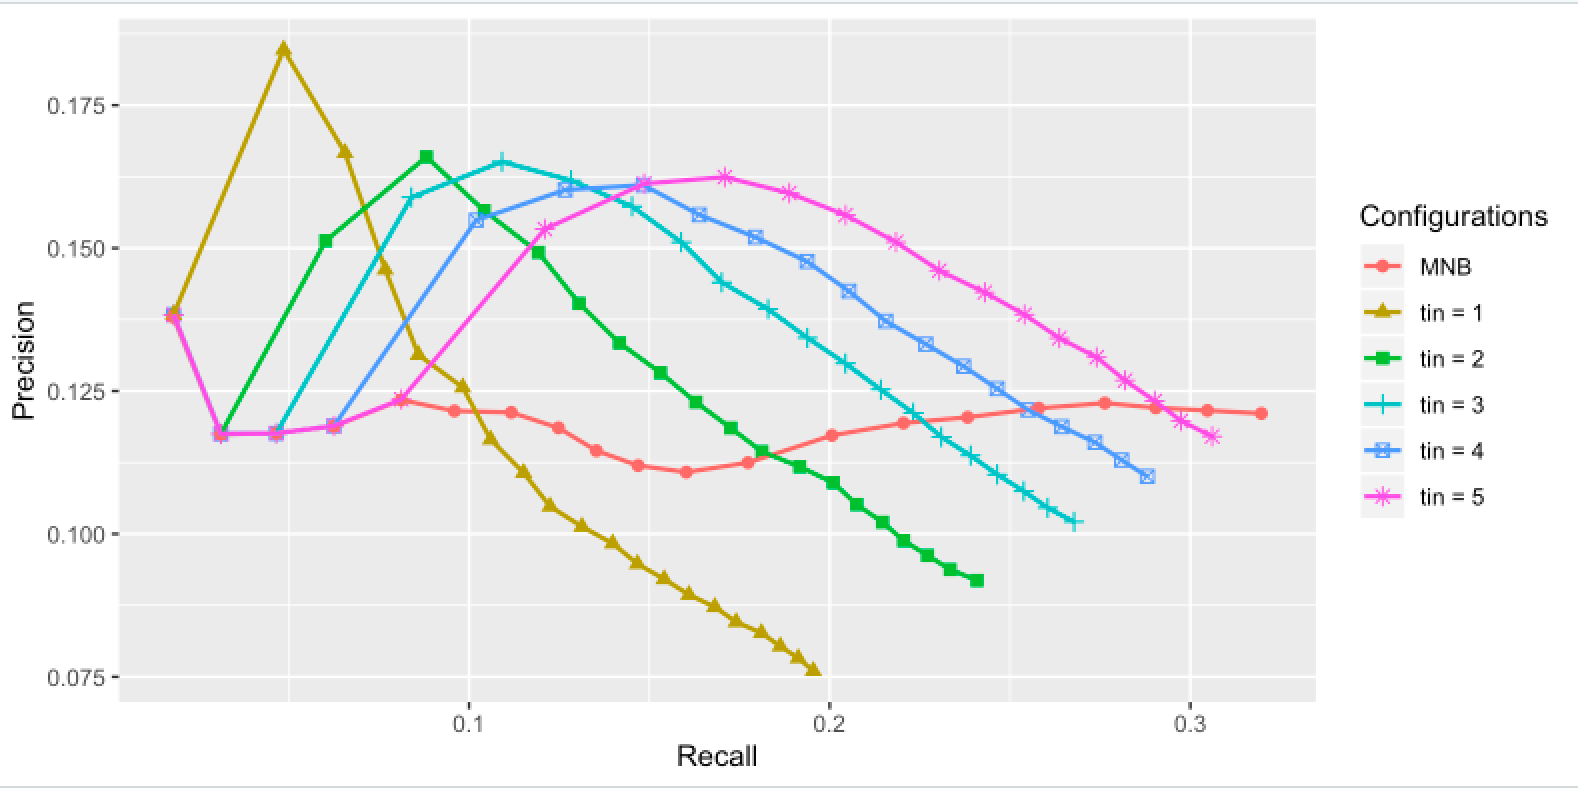
\includegraphics[width=\linewidth]{figs/PRCs_entangled}
%	\caption{Evaluation of the different input topics.}
%	\label{fig:prcs-entangled}
%\end{figure} 


\begin{tcolorbox}[boxrule=0.86pt,left=0.3em, right=0.3em,top=0.1em, bottom=0.05em]
The entangled approach success in improving the prediction performances. By variating both the input and output number of topics, the accuracy and success rate experienced an enhancement even though the former reached low values. The \MNB lacks in catalog coverage, as clearly demonstrated by the higher value of the entangled experiment.
\end{tcolorbox}









%This section reports and discusses the results of our study by addressing the research questions formulated in Section \ref{sec:Evaluation}. \revised{The section is structured into the following subsections.~\Cref{sec:Example} introduces an example of the recommendation results by \LR and \CR.} In~\Cref{sec:ResultAnalysis}, we analyze the obtained results to study the systems' performance. Finally,~\Cref{sec:ThreatsToValidity} discusses the probable threats to validity of our findings. 
%
%
%
%\subsection{Explanatory Example} \label{sec:Example}
%Before addressing our research questions, we illustrate the recommendations of \CR through a running example, \ie the project  \textit{peakgames/libgdx-stagebuilder}  hosted on GitHub.
%As shown in Table \ref{tab:Example}, such a project uses $16$ libraries, which are listed on the left-hand side of the table. Among $16$ included libraries, $8$ items are extracted and used as the ground-truth libraries that are shown in gray. The remaining $8$ items are used as inputs for similarity computation and recommendation, or query. The output obtained by each system is a ranked list in descending order of recommendations with real scores. We took the first $10$ libraries, removed the scores and kept only the order of the list to present the results as in Table~\ref{tab:Example}. The top-$10$ items are then matched against the ground-truth data. 
%%Among $10$ suggested libraries, there are $1$ and $5$ hits by \LR and \CR, respectively, and they are shown in Table~\ref{tab:Example} in bold face. 
%The column \textbf{Freq.} reports the frequency of occurrence of the 
%recommended library, over the set of $1,200$ projects. In this case, \LR 
%only matches \textbf{junit:junit} with the ground-truth (which is obviously used 
%by many projects for testing purposes) but, as we can notice, \CR 
%matches $4$ more projects with the ground-truth. % \MAX{consists or uses?} of
%
%\begin{table}[t!]
	%	\vspace{-.2cm}
	%\caption[Summary]{Recommendation results.}
	%	\vspace{-.4cm}
	%\scriptsize
	\centering	
	\begin{tabular}{|p{0.30cm}|p{6.00cm}|p{0.60cm}|p{4.60cm}|p{0.50cm}|}  \hline		
	a&a&a&a&a
	\end{tabular}	
	\label{tab:Example}
	%\vspace{-.2cm}
\end{table}
%
%Both \LR and \CR obtain a \emph{success rate@10=1.0}. However, \CR has a better \emph{recall@10} compared to \LR as it returns more relevant items (see Eq.~\eqref{eqn:Recall}). Furthermore, among the matches by \CR, $4$ items appear in the top rows of the ranked list, indicating that \CR recommends with a high \emph{precision@N} (see Eq.~\eqref{eqn:Precision}). \LR returns only $1$ relevant item, which means that both \emph{precision@N} and \emph{recall@N} are considerably lower compared to those of \CR. Furthermore, \LR tends to suggest very popular libraries: $6$ out of $10$ items recommended by \LR are used by more than $200$ projects. For instance, besides \textbf{junit:junit}, the second highest frequency item is \textbf{org.slf4j:slf4j-api} ($473/1,200$). By performing an investigation on the outcome of all queries, we realized that \LR usually recommends very popular items. The reasons for such differences are explained in Section~\ref{sec:ResultAnalysis}.
%
%%\PN{This section aims to explain why Novelty is important}
%Four out of five items recommended by \CR have a low frequency of occurrence. For instance, the first item in the 
%ranked list is \textbf{com.badlogicgames.\ gdx:gdx-platform} and this library is included in only $3/1,200$ projects. 
%Referring to Fig.~\ref{fig:NumOfLibsD3}, it is evident that the top $3$ items belong to the long tail, \ie they are 
%extremely unpopular since each is used by only $3$ projects. However, they turn out to be useful as all of them match 
%those stored as ground-truth. In contrast to some existing studies which choose to recommend only popular items to 
%developers \cite{Ponzanelli:2014:MST:2597073.2597077},\cite{Moreno:2015:IUT:2818754.2818860} we see that popularity is not
%a good indicator for selecting a library. This implies that the novelty of a ranked list is important: a system should 
%be able to recommend libraries that are \emph{novel} \cite{Castells_noveltyand}, \ie those that have been rarely seen. 
%In this sense, we expect that \CR can produce good outcomes, not only in terms of success rate and accuracy, but 
%also sales diversity and novelty. 
%
%In summary, for the explanatory example, \CR obtains a comparable success rate, but better accuracy and novelty than \LR. This also confirms that success rate is not sufficient for evaluating the recommendation outcomes. A good recommender system is the one that can maintain a trade-off by improving diversity, novelty but still retaining a good accuracy \cite{Ragone:2017:SLF:3019612.3019837}. Consequently, it is necessary to investigate if this trade-off is guaranteed by \LR and \CR, and this is done in the next sub-sections by considering the whole dataset discussed in the previous section.
%
%
%
%%====================================================================================================================================
%%. In this sense, we see that.  exploit popularity as a means to recommend
%%``long tail''
%%they are far apart from each other in the ranked list, thereby resulting in low precision. %Referring to Table~\ref{tab:FreqDeps}, we see that $7$ out $10$ items recommended by \LR belong to the most popular libraries, whereas the corresponding figure of \CR is $4$. In other words, most of the items recommended by \LR do not fall into the long tail, thus yielding a low novelty for the recommendations.
%
%%According to \emph{Ragone et al.} , 
%%all the testing folds to see
%%\todo[size=\tiny, color=green!40]{Nr. 2: Project without popular 3rd party libs}\footnote{\url{https://github.com/inovait/neatle}}
%%====================================================================================================================================
%%The same set of data is provided as input for \LR and \CR. 
%% (Table \ref{tab:Example})
%%Among other recommended items by \CR which are not a match, \href{https://mvnrepository.com/artifact/commons-collections/commons-collections}{\textbf{commons-collections:commons-collections}} is \emph{"a project to develop and maintain collection classes based on and inspired by the JDK collection framework."} Meanwhile, \href{https://github.com/guoguibing/librec}{\textbf{guoguibing/librec}} is a project that implements various recommendation algorithms. We see that, the library might be useful for the running project.
%%This library we see that
%%and we are going to explain the results in the following sub-sections.  are able to maintain the trade-off
%%Nevertheless, the novelty for this input project is low by both systems. 
%%As already suggested, it is important to maintain a trade-off between. 
%%In a good recommender system there should be a trade-off between accuracy and diversity. diversity should be improved while maintaining adequate accuracy.
%%By manually investigating several queries, we notice that \CR can produce more relevant recommendations in the beginning of the list.
%%Also by comparing with the list of   
%%can recommends the items  %The results are presented in Table \ref{tab:Example}. The asterisk next to the libraries in the third column indicates that it matches against one of the items in the ground-truth libraries. %libraries printed in bold are the matches.
%%\cellcolor{Gray} 
%%====================================================================================================================================
%
%
%
%
%
%
%\subsection{Empirical Study Results} \label{sec:ResultAnalysis}
%
%%\color{blue}
%
%\revised{In this section, we report the results by addressing the research questions \textbf{RQ$_1$}, \textbf{RQ$_2$}, \textbf{RQ$_3$}, \textbf{RQ$_4$}, and \textbf{RQ$_5$}.}
%
%%discrepancies.
%
%\vspace{.1cm}
%%\noindent\textbf{RQ$_1$:} \emph{Does \CR obtain a better success rate compared to \LR?}
%\noindent \revised{\rqfirst}
%\vspace{-.05cm}
%
%%The original dataset consists of. 
%%, (\eg)
%
%
%
%\noindent%N (the cut-off value for the list of items to be recommended) 
%%\emph{Success rate:}  %We are interested in understanding the. We concentrate on comparing \CR with \LR. In the following section.
%%\paragraph{\textbf{Success rate}} 
%% answer this question
%%To compare \CR with \LR, 
%
%
%\paragraph{\textbf{Comparison between \LR and \CR}} We performed a series of experiments on \code{D1} using different combinations of number of recommended libraries (\ie $N$), and number of neighbor projects exploited in the recommendation phase (\ie $k$). Varying $N$ means changing the length of the recommendation list, whereas increasing $k$ means considering more neighbor projects for recommendation.
%
%
%\begin{figure*}[h!]
%	\centering
%	
%	\begin{tabular}{c c}	
%		\centering    
%		\subfigure[Success rate@5, 
%		k=\{5,10,15,20,25\}]{\label{fig:RecallRate5}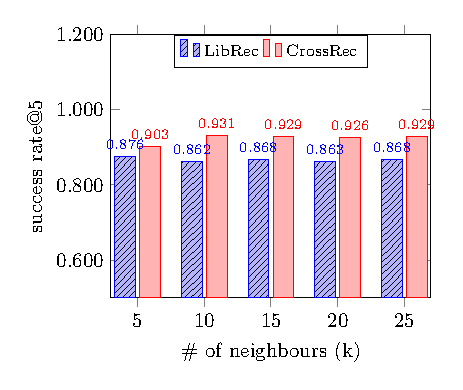
\includegraphics[width=0.48\textwidth]{figs/RecallRate@5.pdf}}		& 	
%		\subfigure[Success rate@10, k=\{5,10,15,20,25\}]{\label{fig:RecallRate10}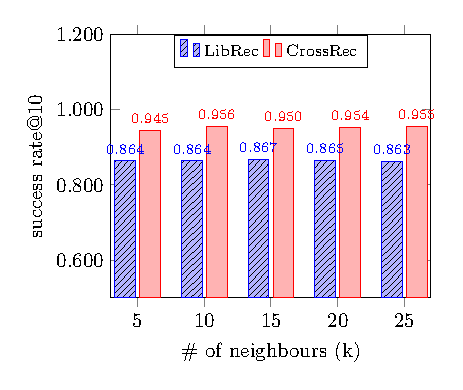
\includegraphics[width=0.48\textwidth]{figs/RecallRate@10.pdf}}\\
%		\subfigure[Success rate@\{1,3,5,7,10\}, k=10]{\label{fig:RecallRateNk10}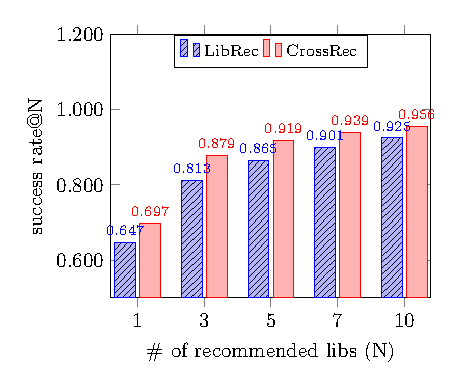
\includegraphics[width=0.48\textwidth]{figs/RecallRate@N_k10.pdf}}	& 	
%		\subfigure[Success rate@\{1,3,5,7,10\}, k=20]{\label{fig:RecallRateNk20}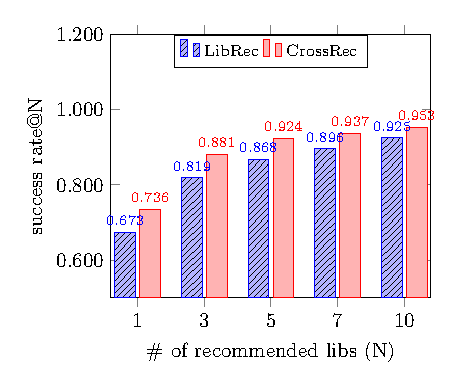
\includegraphics[width=0.48\textwidth]{figs/RecallRate@N_k20.pdf}}\\
%	\end{tabular}
%	\label{fig:RecallRate}
%	\caption{Success rate of \CR and \LR on \code{D1}.}
%\end{figure*}
%
%
%Fig.~\ref{fig:RecallRate5} shows the \emph{success rate@5} for k=\{5, 10, 15, 20, 25\}. As it can be seen there, the success rate values obtained by \CR are always superior to those of \LR. The maximum \emph{success rate@5} of \LR is $0.876$, whereas \CR obtains success rates being greater than $0.903$ for all configurations, with $0.931$ being the maximum value. Fig.~\ref{fig:RecallRate10} shows the \emph{success rate@10}, for this setting, \LR gains a comparable performance for $N=5$. Meanwhile, \CR achieves a slight improvement in its performance compared to the case with $N=5$. It is evident that \CR outperforms \LR in all test configurations. Fig.~\ref{fig:RecallRate5} and Fig.~\ref{fig:RecallRate10} imply that changing the number of neighbor projects $k$ does not make a substantial difference in their match rate, as \emph{success rate@N} is stable towards $k$ for both systems.
%
%Next, we investigate the success rate with regards to $N$. We consider a small number of recommended items, \ie $N=\{1,3,5,7,10\}$. In practice, this means that the developer wants to see a short list of recommended libraries. In the first experiment, $k$ is fixed to $10$ and the outcomes are depicted in Fig. \ref{fig:RecallRateNk10}. For $N=1$, \LR achieves a success rate of $0.647$ which is lower than the corresponding value $0.697$ produced by \CR. A success rate of $0.697$ implies that \CR can supply relevant recommendations to the developer at an encouraging match rate, even when she expects only an extremely brief list. Once $k$ is changed from $10$ to $20$, both systems have a slight increase in \emph{success rate@1} as depicted in Fig. \ref{fig:RecallRateNk20}. However, for other values of $N$, there are almost no changes in success rate. To further observe this behavior, we conducted more experiments with an increasing $k$, \eg $k=\{50,60,100\}$. As far as we can see, there are no subtle differences between the conclusions obtained from the new experiments with those previously presented in the paper. Thus, for the sake of clarity, the outcomes of these experiments are omitted from the paper.
%
%%Nevertheless, the outcomes of these experiments are omitted from the paper due to space limitation. We noticed that considering more similar projects for recommendation does not improve success rate. %When we consider a bigger value of $N$, starting from $N=5$, \CR gains a quick increase in its performance as the success rates are always greater than $0.924$. 
%
%%Last but not least, t
%
%
%%The second column of Table \ref{tab:Wilcoxon} and of Table \ref{tab:Cliff} 
%
%%To see if the improvement of the proposed approach is statistically significant and substantial, we perform a Wilcoxon rank sum test \cite{Wilcoxon1992} on all the quality scores for both systems, using $k=10$ and $N=\{3,5,10,15\}$. The $p$-values for all quality metrics are shown in Table~\ref{tab:Wilcoxon}. The null hypothesis is that there are no differences between the performance of \CR and that of \LR. Using $5\%$ as the confidence level, we see that by all quality indicators the \emph{p-values} are always lower than $5 \times e^{-2}$. Cliff's $d$ values are reported in Table \ref{tab:Cliff}. As the table shows, the observed differences are always in favor of \CR (\ie effect sizes are always positive). Magnitude of the computed Cliff's $d$ is small for precision and recall, while it is large for all other indicators, including Success Rate.
%%
%%\begin{tcolorbox}
%%In this sense, we reject the null hypothesis and conclude that the performance improvement obtained by \CR is statistically significant. %or \emph{p-value} $< 5 \times e^{-2}$ . in terms of all quality metrics. 
%%\end{tcolorbox}
%
%
%\begin{table*}[ht]
%	\footnotesize	
%	\color{blue}
%	\caption{Wilcoxon rank sum test adjusted $p$-values and Cliff's $d$ results for N=\{3,5,10,15\}, k=10.}
%	\centering
%	\begin{tabular}{|p{4.3cm}|p{1.0cm}|p{1.0cm}|p{1.0cm}|p{1.0cm}|}\hline
%	%	\rowcolor{verylightgray}
%		& \multicolumn{4}{c|}{\textbf{Cut-off value (N)}}         \\ \hline
%		\textbf{Test} & 3	 & 5   & 7     & 10    \\ \hline
%		Wilcoxon r.s.t. adjusted $p$-values  & 0.02 & 0.02 & 0.17 & 0.002  \\ \hline
%		Cliff's $d$ results   &  0.70 (l) & 0.74 (l) & 0.93 (l) & 0.58 (l) \\ \hline
%	\end{tabular}
%	\label{tab:WilcoxonCliffLibRecCrossRec}
%	\color{black}
%\end{table*}
%
%\revised{Table \ref{tab:WilcoxonCliffLibRecCrossRec} reports Wilcoxon rank sum test adjusted $p$-values and Cliff's $d$, respectively for the comparison of \LR and \CR in terms of {\em success rate}, using $k=10$ and $N=\{3,5,10,15\}$; the labels in parentheses indicate the magnitude (n:negligible, s:small, l:large). As the table shows, the differences are always statistically significant and in favor of \CR (effect size is positive), with a large effect size.}
%
%
%\begin{tcolorbox}[boxrule=0.86pt,left=0.3em, right=0.3em,top=0.1em, bottom=0.05em]
%	%	\color{blue}
%	%	\revised{
%	\small{In summary,  \CR significantly outperforms \LR in all considered test configurations concerning \emph{success rate}, with a large effect size. The recommendation time for a fold (120 projects) is relatively faster for \CR (3s) than for \LR (20s).}%}%  \CR can reach a high performance when.
%\end{tcolorbox}
%
%
%
%%We also measured the average time needed to generate, 
%%We analyzed the dataset\footnote{\url{http://sel.ist.osaka-u.ac.jp/people/ali/libRecommendation/}} exploited to evaluate \LF~\cite{Ouni:2017:SSL:3032135.3032325}. 
%%We varied the number
%%on-the-fly’ recommendations in such a way that the developer will be automatically notified by relevant libraries while he is writing his code
%%|p{0.8cm}|
%%\LF was evaluated using different metrics, however in our work we are interested in comparing. 
%
%%We performed experiments on \code{D2} to. 
%% when N increases
%%a high performance is favored and helps developers approach relevant libraries
%
%\paragraph{\textbf{\revised{Comparison between \LF and \CR}}} \revised{Even though \LF is a bit different from \CR as it aims at providing \emph{on-the-fly} recommendations while the developer is coding by exploiting the existing semantic, we attempted to compare \CR with \LF by applying the same experimental settings. A comparison between \LF and \CR is depicted in Table~\ref{tab:SuccessRateLibFinderCrossRec}.\footnote{\revised{The success rates of \LF were extracted directly from the paper~\cite{Ouni:2017:SSL:3032135.3032325}}.} For small cut-off values, \ie $N=\{1,2,4\}$, \CR obtains a better success rate than \LF does. However, by the higher values $N=\{6,8,10\}$, \LF gains an improvement in its performance. This suggests that \LF tends to provide matches quite late in the ranked list. On one hand, a system with such a recommendation list helps developers approach relevant libraries. On the other hand, this is not useful for those who prefer to get only a short list of recommendations.}
%
%
%%\revised{
%\begin{table*}[ht]
%	\footnotesize	
%	\color{blue}
%	\caption{Success rate of \LF and \CR on \code{D2}.}
%	\centering
%	\begin{tabular}{|p{1.5cm}|p{1.0cm}|p{1.0cm}|p{1.0cm}|p{1.0cm}|p{1.0cm}|p{1.0cm}|}\hline
%		%\rowcolor{grey}
%		& \multicolumn{6}{c|}{\textbf{Cut-off value (N)}}         \\ \hline
%		\textbf{System} & 1	 & 2   & 4      & 6   & 8    &  10          \\ \hline
%		\LF  & 0.633 & 0.698 & 0.813 & \textbf{0.876} & \textbf{0.904} & \textbf{0.918}  \\ \hline
%		\CR  & \textbf{0.771} & \textbf{0.816} & \textbf{0.851} & 0.860 & 0.863 & 0.864  \\ \hline
%	\end{tabular}
%	\label{tab:SuccessRateLibFinderCrossRec}
%	\color{black}
%\end{table*}
%%}
%
%% with a certain level of maturity
%% which cannot be used as input for the splitting
%% with different levels of maturity
%
%\revised{By carefully examining the \code{D2} dataset, we realized that there are several projects containing a small number of dependencies, \eg 1 or 2 third-party libraries. Such projects are not beneficial to the training of \CR since the corresponding metadata is not sufficient to compute similarity and, consequently, to provide a recommendation (see Eq.~\eqref{eqn:TFIDF} and Eq.~\eqref{eqn:VsmSim}). Thus, to further investigate the performance of \CR on~\code{D2}, we performed a filtering step as follows. Starting from the dataset, we selected projects containing a certain number of libraries, and such a number is called as $L$. The number was then varied to create different configurations. In practice, this means that we consider only mature projects, \ie those that include a decent number of libraries for training. Table~\ref{tab:SuccessRateCrossRecD1} shows the success rate obtained by varying $L$. As it can be seen, CrossRec's performance is proportional to $L$: the more dense (with respect to dependencies) the projects are, the better performance \CR achieves. For instance, when we consider only projects with at least $4$ libraries, \ie $L=4$ the success rate obtained for $N=10$ is $0.914$. However, if $L$ is increased to $10$, the corresponding success rate improves to reach $0.987$. The same trend can be witnessed by other combinations of $L$ and $N$.} %Thus, the first conclusion to be drawn is that \CR is able to work on a large datasets and provide accurate recommendations.} % achieves much better performance when.
%
%%\revised{
%\begin{table*}[ht]
%	\footnotesize
%	\color{blue}
%	\caption{Success rate of \CR on \code{D2} with different number of libraries ($L$).}
%	\centering
%	%	\begin{tabular}{|r|r|r|r|r|r|r|}\hline
%	\begin{tabular}{|p{0.75cm}|p{0.75cm}|p{1.0cm}|p{1.0cm}|p{1.0cm}|p{1.0cm}|p{1.0cm}|p{1.0cm}|}\hline
%		%\rowcolor{verylightgray}
%		\multicolumn{2}{|c|}{} & \multicolumn{6}{c|}{\textbf{Cut-off value (N)}}         \\ \hline%\cline{3-8}
%		%		\rowcolor{verylightgray}
%		\multicolumn{2}{|c|}{\textbf{\# of libraries}} & 1	 & 2   & 4    & 6   & 8    &  10          \\ \hline
%		{\multirow{4}{*}{$L$}} & 4          & 0.811 & 0.853 & 0.894 & 0.906 & 0.911 & 0.914  \\ \cline{2-8}
%		& 6          & 0.890 & 0.926 & 0.948 & 0.958 & 0.961 & 0.964  \\ \cline{2-8}
%		& 8          & 0.930 & 0.958 & 0.972 & 0.977 & 0.982 & 0.986  \\ \cline{2-8}
%		& 10         & 0.938 & 0.964 & 0.976 & 0.981 & 0.984 & 0.987  \\ \hline
%	\end{tabular}
%	\label{tab:SuccessRateCrossRecD1}
%	%\vspace{-.1cm}
%	\color{black}
%\end{table*}
%%}
%
%
%%=====================================================================================
%% has been neglected by LibFinder
%%Finally, we also incorporate libraries' version. 
%% is not used in the evaluation
%%which is a limitation of LibFinder. 
%%neglects 
%%The final dataset consists of 5,102 projects and. 
%%Furthermore, \CR is able to recommend library version, 
%%as stated in the original paper~\cite{Ouni:2017:SSL:3032135.3032325}
%%\CR transcends the limitation of \LF since it is capable of recommending libraries with versions. Moreover, \CR obtains a better performance when the input data is dense, \ie more libraries are available for training.
%%We come to the conclusion that o
%%in Table~\ref{tab:SuccessRateCrossRecD2Version}
%%=====================================================================================
%
%
%\revised{While the \code{D2} dataset also specifies library versions,
%	\LF is unable to deal with this information, resulting in a limitation, as already stated by the authors~\cite{Ouni:2017:SSL:3032135.3032325}. In practice, it is crucial to provide developers with not only a suitable library, but also a specific version of that library, otherwise there might be some issues related to version compatibility~\cite{Mileva:2009:MTL:1595808.1595821} or, in general, recommending obsolete libraries. Thus, we injected also library version into the training and testing data and fed it to \CR. The final results for different configurations are reported in Table~\ref{tab:SuccessRateCrossRecD2Version}.} \revised{As it can be seen in the table, given that decent training data is available, \CR also recommends libraries with version, achieving a high success rate. For instance, even when projects containing at least 2 libraries are considered, or $L=2$, \CR obtains a success rate of $0.620$ for $N=1$. This quality metric improves linearly alongside $L$ and $N$. As an example, when $L=10$ and $N=10$, the corresponding success rate is $0.955$.}
%
%
%
%	\begin{table*}[ht]
%		\footnotesize
%		\color{blue}
%		\caption{Success rate of \CR on \code{D2} when library version is considered.}
%		\centering
%		%	\begin{tabular}{|r|r|r|r|r|r|r|}\hline
%		\begin{tabular}{|p{0.75cm}|p{0.75cm}|p{1.0cm}|p{1.0cm}|p{1.0cm}|p{1.0cm}|p{1.0cm}|p{1.0cm}|}\hline
%%			\rowcolor{gray}
%			\multicolumn{2}{|c|}{} & \multicolumn{6}{c|}{\textbf{Cut-off value (N)}}         \\ \hline%\cline{3-8}
%			%		\rowcolor{verylightgray}
%			\multicolumn{2}{|c|}{\textbf{\# of libraries}} & 1	 & 2   & 4    & 6   & 8    &  10          \\ \hline
%			{\multirow{4}{*}{$L$}} & 2 	& 0.620 & 0.676 & 0.715 & 0.729 & 0.735 & 0.738  \\ \cline{2-8}
%			& 4                    		& 0.785  & 0.834 & 0.872 & 0.893 & 0.903 & 0.907  \\ \cline{2-8}
%			& 6                    		& 0.848 & 0.885  & 0.907 & 0.921 & 0.931 & 0.936  \\ \cline{2-8}
%			& 8                    		& 0.888 & 0.919 & 0.931 & 0.937 & 0.945 & 0.950  \\ \cline{2-8}
%			& 10                   		& 0.906 & 0.930 & 0.944 & 0.948 & 0.951 & 0.955  \\ \hline
%		\end{tabular}
%		\label{tab:SuccessRateCrossRecD2Version}
%		\color{black}
%		%\vspace{-.1cm}
%	\end{table*}
%
%
%\begin{tcolorbox}[boxrule=0.86pt,left=0.3em, right=0.3em,top=0.1em, bottom=0.05em]
%	%	\color{blue}
%	\revised{
%		\small{On the \code{D2} dataset, \CR obtains a comparable performance compared to that of \LF. When it comes to a dataset containing projects with more libraries, \CR is able to give more precise recommendations. Differently from \LF, \CR is capable recommending also a specific version of a library.}}
%\end{tcolorbox}
%
%
%
%
%
%
%\paragraph{\textbf{\revised{Comparison between \LC and \CR}}} \revised{For this 
%	evaluation, we used the same experimental settings utilized to evaluate \LF. In 
%	particular, the following cut-off values have been considered: 
%	$N=\{1,3,5,7,10\}$. According to Table~\ref{tab:SuccessRateD2}, the performance 
%	obtained by \CR is always better than that of \LC.\footnote{\revised{The 
%			success rate values for \LC were extracted from the 
%			paper~\cite{SAIED2018164}}.} For example, when the cut-off value $N=1$, \LC 
%	gets $0.12$ as success rate while the corresponding value by \CR is $0.21$. 
%	Similarly, for other values of $N$, our proposed tool gains a superior 
%	performance compared to that of \LC, in particular when $N=10$, \CR achieves a 
%	success rate which is nearly twice what \LC achieves, \ie $0.42$ compared to 
%	$0.22$.}% \MAX{this is the only case where success rate has 2 digits instead of 
%%3. Maybe because of the data in the original paper?}} \PN{Yes, you are right. 
%%In the original paper, we can find only scores with two digits.}
%
%
%\begin{table*}[ht]
%	\footnotesize
%	\color{blue}
%	\caption{Success rate of \LC and \CR on \code{D3}.}
%	\centering
%	\begin{tabular}{|p{1.5cm}|p{1.0cm}|p{1.0cm}|p{1.0cm}|p{1.0cm}|p{1.0cm}|}\hline
%%		\rowcolor{verylightgray}
%		& \multicolumn{5}{c|}{\textbf{Cut-off value (N)}}         \\ \hline
%		\textbf{System} & 1	 & 3   & 5      & 7   & 10          \\ \hline
%		\LC  & 0.12 & 0.14 & 0.15 & 0.17 & 0.22   \\ \hline
%		\CR  & \textbf{0.21} & \textbf{0.31} & \textbf{0.36} & \textbf{0.39} & \textbf{0.42}   \\ \hline
%	\end{tabular}
%	\label{tab:SuccessRateD2}
%\end{table*}
%
%
%\revised{Similarly to \code{D2}, \code{D3}  also features library versions, however \LC cannot provide version-specific recommendations. For each library in the dataset, we integrated its version and fed as input for \CR. For this experiment, we selected only projects with a considerably high number of third-party libraries, \ie $L=\{7,8,9,10\}$ and the final results are shown in Table~\ref{tab:SuccessRateCrossRecD3Version}.}
%
%
%%\revised{To conform with. For this evaluation, we also. The following cut-off values have been considered: $N=\{1,3,5,7,10\}$. According to Table~\ref{tab:SuccessRateD2}, the performance obtained by \CR is always better than that of \LC. For example, when the cut-off value $N=1$, \LC gets $0.12$ as success rate while the corresponding value by \CR is $0.21$. Similarly, for other values of $N$, \CR gains a superior performance compared to \LC, for example when $N=10$.}
%
%
%	\begin{table*}[ht]
%		\footnotesize
%		\color{blue}
%		\caption{Success rate of \CR on \code{D3} when library version is incorporated.}
%		\centering
%		\begin{tabular}{|p{0.75cm}|p{0.75cm}|p{1.0cm}|p{1.0cm}|p{1.0cm}|p{1.0cm}|p{1.0cm}|}\hline
%%			\rowcolor{verylightgray}
%			\multicolumn{2}{|c|}{} & \multicolumn{5}{c|}{\textbf{Cut-off value (N)}}         \\ \hline%\cline{3-8}
%			\multicolumn{2}{|c|}{\textbf{\# of libraries}} & 1	 & 3   & 5    & 7   & 10          \\ \hline
%			{\multirow{4}{*}{$L$}} & 7 	& 0.215 & 0.313 & 0.361 & 0.392 &  0.423  \\ \cline{2-7}
%			& 8                    		& 0.219 & 0.315 & 0.362 & 0.392 & 0.423   \\ \cline{2-7}
%			& 9                    		& 0.214 & 0.311 & 0.355 & 0.383 &  0.415  \\ \cline{2-7}
%			& 10                        & 0.255 & 0.368 & 0.422 & 0.456 &  0.494  \\ \hline
%		\end{tabular}
%		\label{tab:SuccessRateCrossRecD3Version}
%		\color{black}
%	\end{table*}
%
%%As it can be seen in Table~\ref{tab:SuccessRateCrossRecD3Version}, 
%%the same trend can be witnessed: 
%%Given that decent training data is available, 
%%According to 
%% For instance, even when projects containing at least 2 libraries are considered, or $L=2$, \CR obtains a success rate of $0.620$ for $N=1$.
%% the success rates are.
%% is very small
%
%\revised{Table~\ref{tab:SuccessRateCrossRecD3Version} shows that \CR also recommends specific versions of libraries. Among the configurations, the maximum success rate is $0.494$, and it is reached when $L=10$ and $N=10$. However, in comparison to the outcome by \code{D2}, \CR achieves a considerably lower success rate. Moreover, there is a marginal difference in performance between different values of $L$. Especially, the system's performance suffers a setback when $L=9$ in comparison to $L=8$. By carefully investigating the dataset, we found out that the projects of \code{D2} are very diverse, and they contain a large number of libraries. Moreover, the similarity among the projects is considerably low. This means that the dataset exhibits a high level of heterogeneity and therefore, given a project, generally we cannot find a good set of similar projects. Under the circumstances, it is more difficult to recommend highly relevant libraries, resulting in a low success rate.}
%
%
%%A possible explanation for this is that 
%
%%\begin{tcolorbox}[boxrule=0.86pt,left=0.3em, right=0.3em,top=0.1em, bottom=0.05em]
%%%	\color{blue}
%%	\revised{\small{On the \code{D2} dataset, \CR clearly outperforms \LC. \CR can reach a better performance when.}}
%%\end{tcolorbox}
%
%
%\begin{tcolorbox}[boxrule=0.86pt,left=0.3em, right=0.3em,top=0.1em, bottom=0.05em]
%	\revised{\small{On the \code{D3} dataset, \CR clearly outperforms \LC with respect to various configurations. Furthermore, \CR can recommend also libraries with a specific version, which \LC cannot.}}
%\end{tcolorbox}
%
%
%%====================================================================================================================================
%%filter out the data and retain those projects that.
%
%%\begin{table*}[t]
%%	\footnotesize
%%	\caption{Wilcoxon rank sum test p-values for N=\{3,5,10,15\}, k=10}
%%	\vspace{-.3cm}
%%	\centering
%%	\begin{tabular}{|p{0.5cm}||p{1.60cm}|p{1.80cm}|p{1.50cm}|p{1.50cm}|p{1.50cm}|p{1.50cm}|}
%%		\hline
%%		& \textbf{Success Rate} &     \multicolumn{2}{c|}{\textbf{Accuracy}}      &   \multicolumn{2}{c|}{\textbf{Sales Diversity}}   & \textbf{Novelty}      \\ \hline
%%		\textbf{N} & Success Rate          & Precision               & Recall                & Coverage                  & Entropy               & EPC                   \\ \hline
%%		3          & $8.87 \times e^{-3}$  & $< 2.20 \times e^{-16}$ & $ 5.40 \times e^{-8}$ & $ 1.29 
%%		\times e^{-4}$  & $ 4.33 \times e^{-5}$ & $ 1.08 \times e^{-5}$ \\ \hline
%%		5          & $6.32 \times e^{-3}$  & $< 2.20 \times e^{-16}$ & $3.03 \times e^{-12}$ & $ 4.87 
%%		\times e^{-4}$  & $ 2.16 \times e^{-5}$ & $ 1.08 \times e^{-5}$ \\ \hline
%%		%7         & $4.34 \times e^{-2}$  & $< 2.20 \times e^{-16}$ & $1.58 \times e^{-10}$ & $ 2.08 
%%		%\times e^{-3}$ & $ 2.16 \times e^{-5}$ & $ 7.57 \times e^{-5}$ \\ \hline
%%		10         & $3.69 \times e^{-2}$  & $< 2.20 \times e^{-16}$ & $4.53 \times e^{-12}$ & $ 1.50 
%%		\times e^{-3}$  & $ 1.08 \times e^{-5}$ & $ 7.57 \times e^{-5}$ \\ \hline
%%		15         & $2.87 \times e^{-2}$  & $ 1.10 \times e^{-14}$  & $5.20 \times e^{-10}$ & $ 1.50 
%%		\times e^{-3}$  & $ 2.16 \times e^{-5}$ & $ 2.05 \times e^{-4}$ \\ \hline
%%	\end{tabular}
%%	\vspace{-.2cm}
%%	\label{tab:Wilcoxon}
%%	\vspace{-.2cm}
%%\end{table*}
%%====================================================================================================================================
%
%
%
%
%
%%====================================================================================================================================
%%phenomenon
%%Also in this experiment setting, \CR overtakes \LR concerning recall rate.% as its recall rates. Once we consider Fig. \ref{fig:RecallRateNk10} and Fig. \ref{fig:RecallRateNk20} together,    
%
%%The results obtained from the experiments  are shown in Fig. \ref{fig:RecallRate}. Specifically, Fig. \ref{fig:RecallRate5} and Fig. \ref{fig:RecallRate10} show the \emph{recall rate@5} and \emph{recall rate@10} for $k=\{5,10,15,20,25\}$.  Fig. \ref{fig:RecallRateNk10}, and Fig. \ref{fig:RecallRateNk20}.
%%The value $N=1$ means the developer needs a single library from the recommendation.
%% starting from $N=5$, the recall rates by \CR are always greater than $0.90$.
%%Table \ref{tab:Tenfold_Neighbours} and \ref{tab:Tenfold_Libraries}. Table \ref{tab:Tenfold_Neighbours} lists the average \emph{recall rate@N} for \emph{N=5} and \emph{N=10} with the number of neighbour projects used for recommendation being varied according to \LR, \ie $k=\{5,10,15,20,25\}$. As can be seen, for all combinations of \emph{k} and \emph{N} using either user-based or item-based collaborative filtering, \CR always earns recall rates that are superior to those of \LR. Specifically, for \emph{N=5}, the recall rates range from $0.88$ to $0.92$ by user-based collaborative filtering and from $0.86$ to $0.91$ by item-based collaborative filtering. Referring back to \cite{6671293}, the maximum \emph{recall rate@10} obtained by \LR with the same test configuration is $0.852$ which is inferior to those obtained by \CR. Similarly, for \emph{k=10}, \CR also outperforms \LR as the maximum \emph{recall rate@10} of VsmSim is $0.94$ whereas the corresponding value by \LR is $0.894$.
%%Even when only $5$ neighbour projects are used as input for recommendation, meaning that the \textbf{Recommendation Engine} has very little clue about the test project, \CR still gives a recall rate of $0.88$. This is the minimum value obtained from this test configuration, however it is still better than the best outcome of \LR which is $0.852$.
%%====================================================================================================================================
%% and. %, which is indeed a high score.
%%\begin{table}[h!]w
%%		n		& k=5       & k=10 		\\ \hline	
%%		10      & 0.92      & 0.94      \\ \hline
%%		20      & 0.91      & 0.94      \\ \hline
%%		50      & 0.91      & 0.94      \\ \hline
%%		60      & 0.91      & 0.95      \\ \hline
%%		100     & 0.90      & 0.93      \\ \hline
%%	\end{tabular}
%%	\caption{Average Recall Rate@k for ten-fold cross validatione
%%	\label{tab:Tenfold}
%%\end{table}
%%====================================================================================================================================
%%Next, we consider different number of neighbours, for $k=5$ and $k=10$, the same number of neighbours as in \LR.  different values of $k$ 
%%In conformance with the evaluation performed in \cite{6671293}, we investigate the performance of the system with regards to the number of recommended libraries, \ie $k=\{1,3,5,7,10\}$ and the results are shown in Table \ref{tab:Tenfold_Libraries}. Also in this experiment \CR obtains better recall rates compared to those of \LR. For the case when $N=1$, meaning that the developer wants to see only one library in the recommendation list, \CR still gets a $recall$ $rate@1=0.69$ by user-based collaborative filtering and $0.68$ by item-based collaborative filtering, respectively. These values are higher compared to $0.616$ by \LR. For $N=3$, \CR has a recall rate of $0.89$ which is higher than $0.804$, the corresponding value in \LR. 
%%Taking the best outcomes obtained by \CR, we depict in Fig. \ref{fig:RecallRateK} and Fig. \ref{fig:RecallRateN} together with the results by \LR. The scores for \LR are extracted from the original \LR paper \cite{6671293}.
%%====================================================================================================================================
%%\begin{figure}[h!]
%%	\centering
%%	\includegraphics[width=0.35\textwidth]{figs/RecallRate.pdf}
%%	\caption{Comparison of recall rate@5 for \LR and \CR}
%%	\label{fig:RecallRate5}
%%\end{figure}
%
%%\begin{figure*}[h!]
%%	\centering
%%	\scriptsize
%%	\centering
%%	\subfigure[]{\label{fig:RecallRate}		
%%		\includegraphics[width=0.35\textwidth]{figs/RecallRate.pdf}
%%		\includegraphics[width=0.35\textwidth]{figs/RecallRateN.pdf}		
%%	}
%%	\caption{Comparison of recall rate@5 for \LR and \CR}
%%	\label{fig:ComparedRecallRate}
%%	\vspace*{-5mm}
%%\end{figure*}
%%====================================================================================================================================
%
%
%
%
%%====================================================================================================================================\\
%%Comparison of \LR and \CR with respect to
%% for \LR and \CR
%%starting from $k=5$, 
%%By increasing the number of neighbour projects from $k=10$ to $k=20$, 
%%its counterpart 
%
%%\begin{table}[h!]
%%	\centering
%%	\begin{tabular}{|p{0.8cm}||p{1.2cm}|p{1.2cm}||p{1.2cm}|p{1.2cm}|} \hline		
%%		& \multicolumn{2}{|c||}{\textbf{k=10}}  & \multicolumn{2}{|c|}{\textbf{k=20}} \\ \hline
%%	\textbf{N}	& \LR    & \CR  & \LR    & \CR	  \\ \hline			
%%		1      & 0.	& 0.  & 0. & 0.     \\ \hline
%%		3      & 0.	& 0.  & 0. & 0.    \\ \hline
%%		5      & 0.	& 0.  & 0. & 0.    \\ \hline
%%		7      & 0.	& 0.  & 0. & 0.    \\ \hline
%%		10     & 0.	& 0.  & 0. & 0.    \\ \hline
%%	\end{tabular}
%%	\caption{Ten-fold cross validation: Average recall rate@N for N=\{1,3,5,7,10\}}
%%	\label{tab:Tenfold_Libraries}
%%\end{table}
%%, implying that it has.  we consider another metric. Since recall rate@k is superficial. 
%%By changing the similarity metric in Module 2 (Fig. \ref{fig:\CR}) 
%% using their source code
%%Similar to the experiments in \LR, we also vary the training dataset to investigate the effect. We
%%Varying training set. %Varying recommendation size
%%We used a dataset collected from GitHub using the provided API.
%%Thus, it is worth comparing against RepoPal. 
%%We apply the same recommendation engine (Module 3), thus to validate the similarity computation modul. %As a result, we consider RepoPal as a good reference for similarity computation technique. 
%% as it obtains better quality metrics in comparison with CLAN
%%The results in Table \ref{tab:Tenfold_Neighbours} and Table \ref{tab:Tenfold_Libraries} demonstrate that in comparison to \LR, \CR is always able to generate a better recommendation to a given project, with regards to \emph{recall rate@N}. In summary, by using the same evaluation methodology as well as (almost) the same dataset, we see that \CR considerably outperforms \LR.
%%====================================================================================================================================
%
%
%%\begin{figure*}[t!]
%%	%	\vspace{-.4cm}
%%	\begin{tabular}{c c}	
%%		\centering    
%%		\vspace{-.37cm}	
%%		\subfigure[Fold 1]{\label{fig:PrecisionRecallFold1}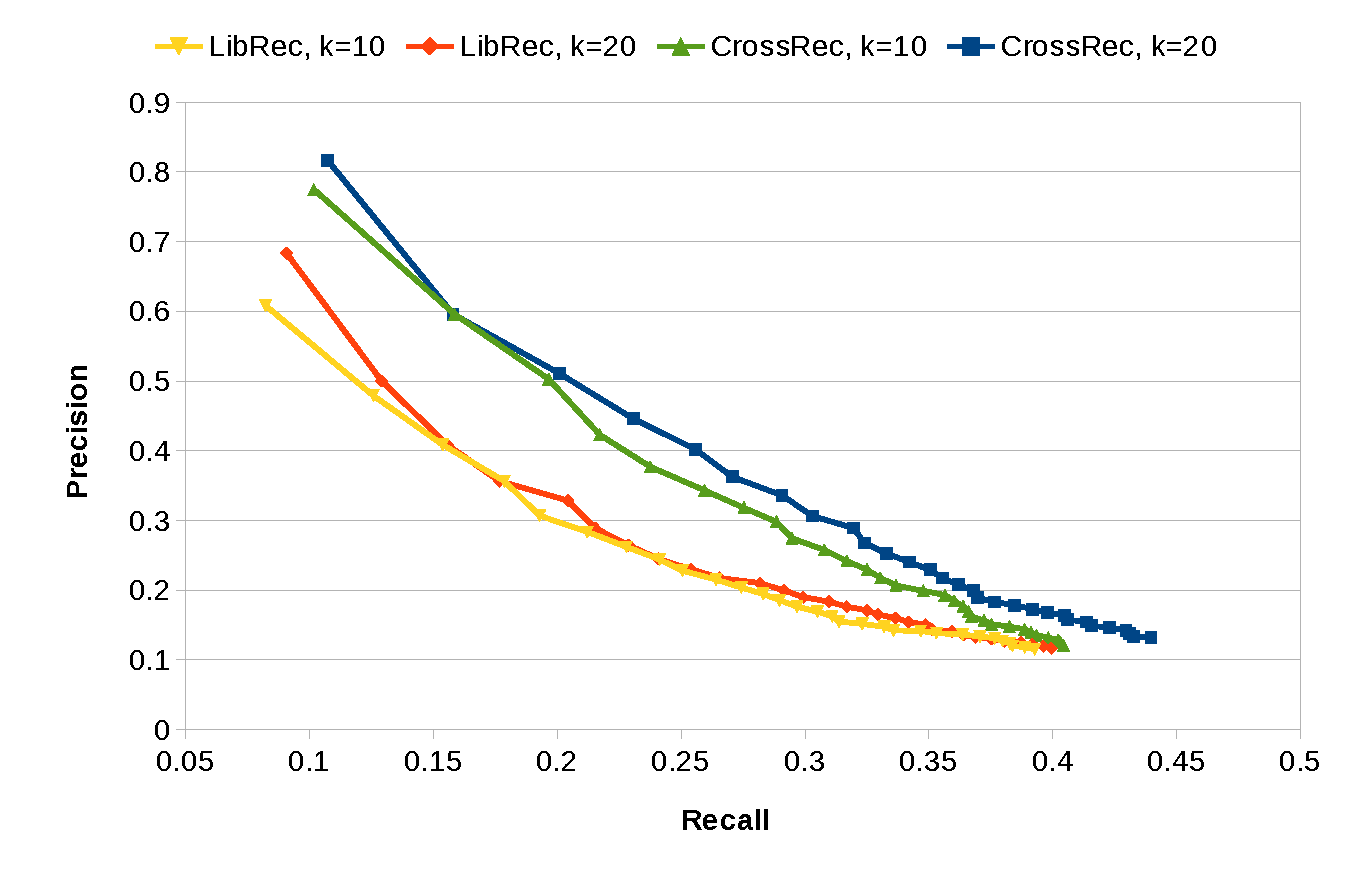
\includegraphics[width=0.45\textwidth]{figs/PrecisionRecall_Fold1.pdf}} & 	
%%		\subfigure[Fold 2]{\label{fig:PrecisionRecallFold2}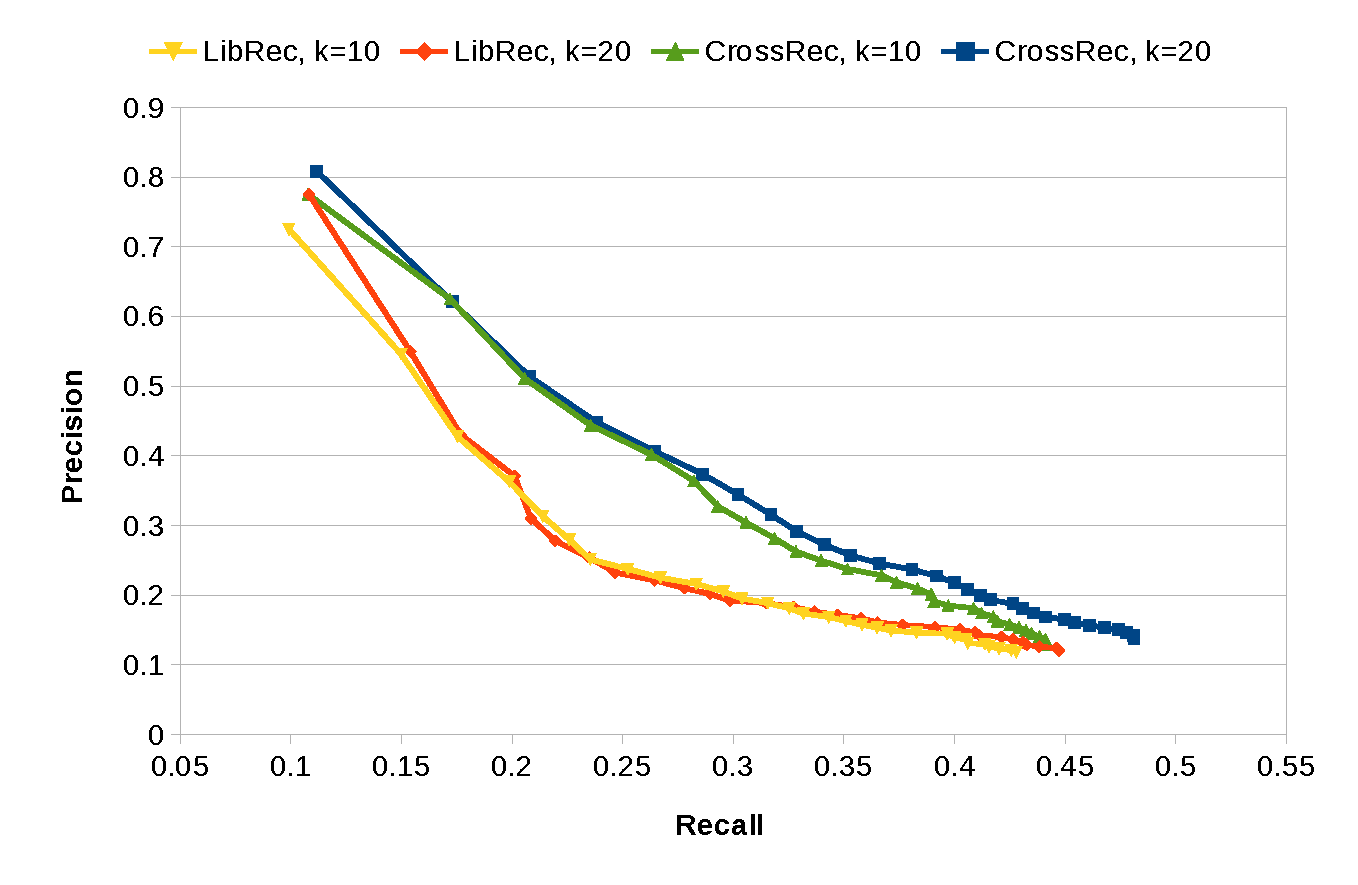
\includegraphics[width=0.45\textwidth]{figs/PrecisionRecall_Fold2.pdf}} \\	
%%		\vspace{-.37cm}	
%%		\subfigure[Fold 3]{\label{fig:PrecisionRecallFold3}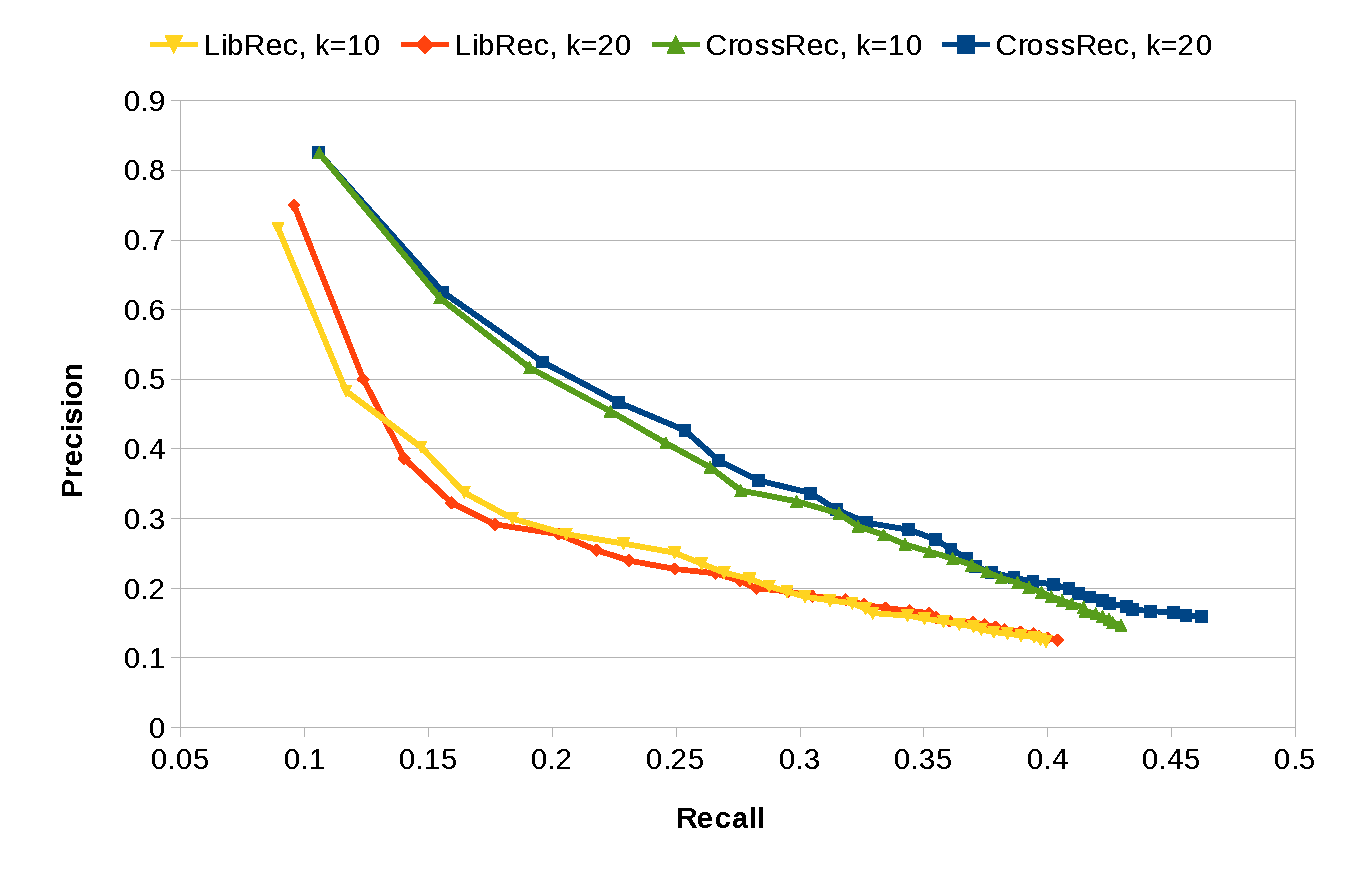
\includegraphics[width=0.45\textwidth]{figs/PrecisionRecall_Fold3.pdf}} & 	
%%		\subfigure[Fold 4]{\label{fig:PrecisionRecallFold4}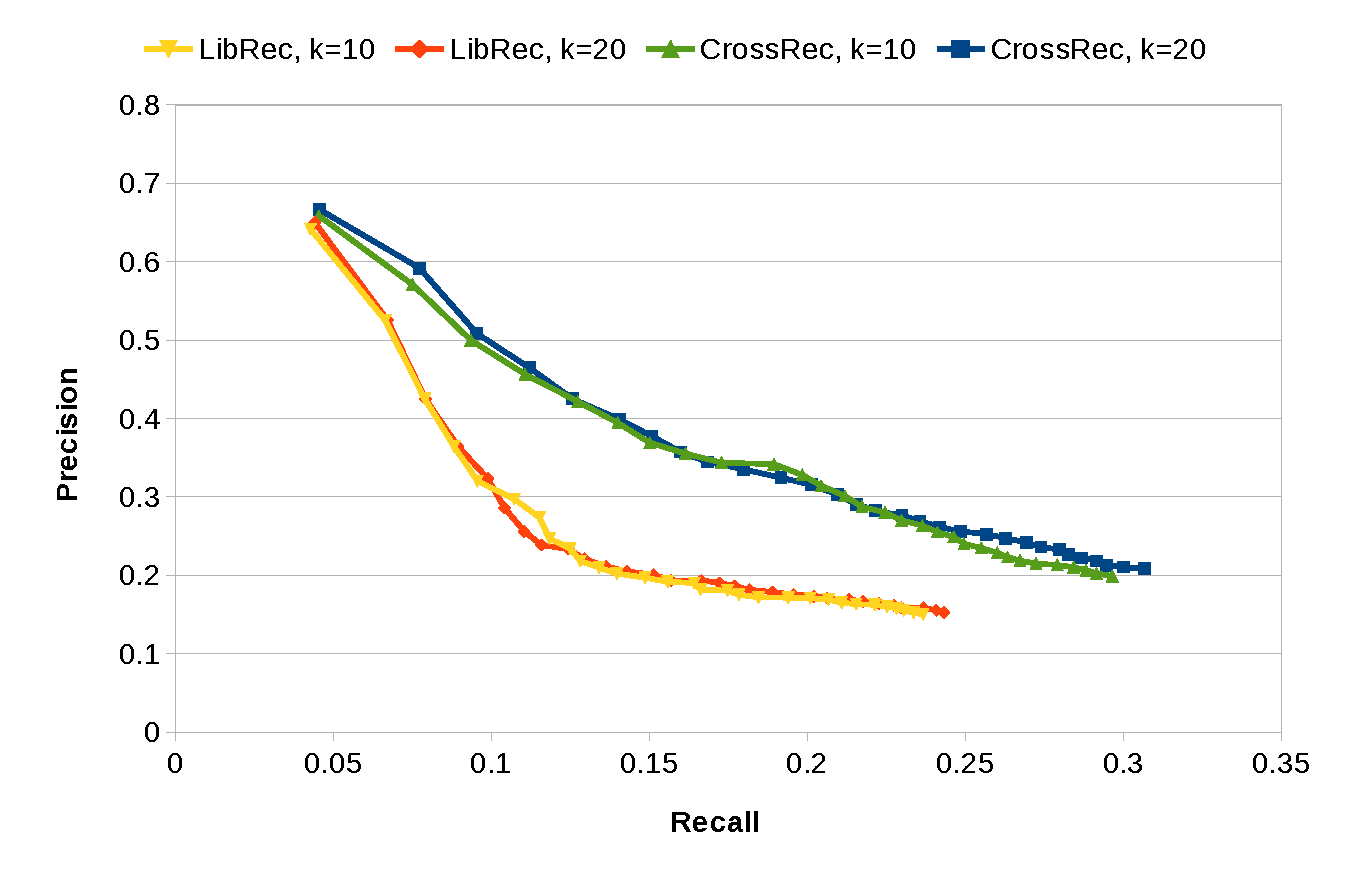
\includegraphics[width=0.45\textwidth]{figs/PrecisionRecall_Fold4.pdf}} \\	
%%		\vspace{-.37cm}	
%%		\subfigure[Fold 5]{\label{fig:PrecisionRecallFold5}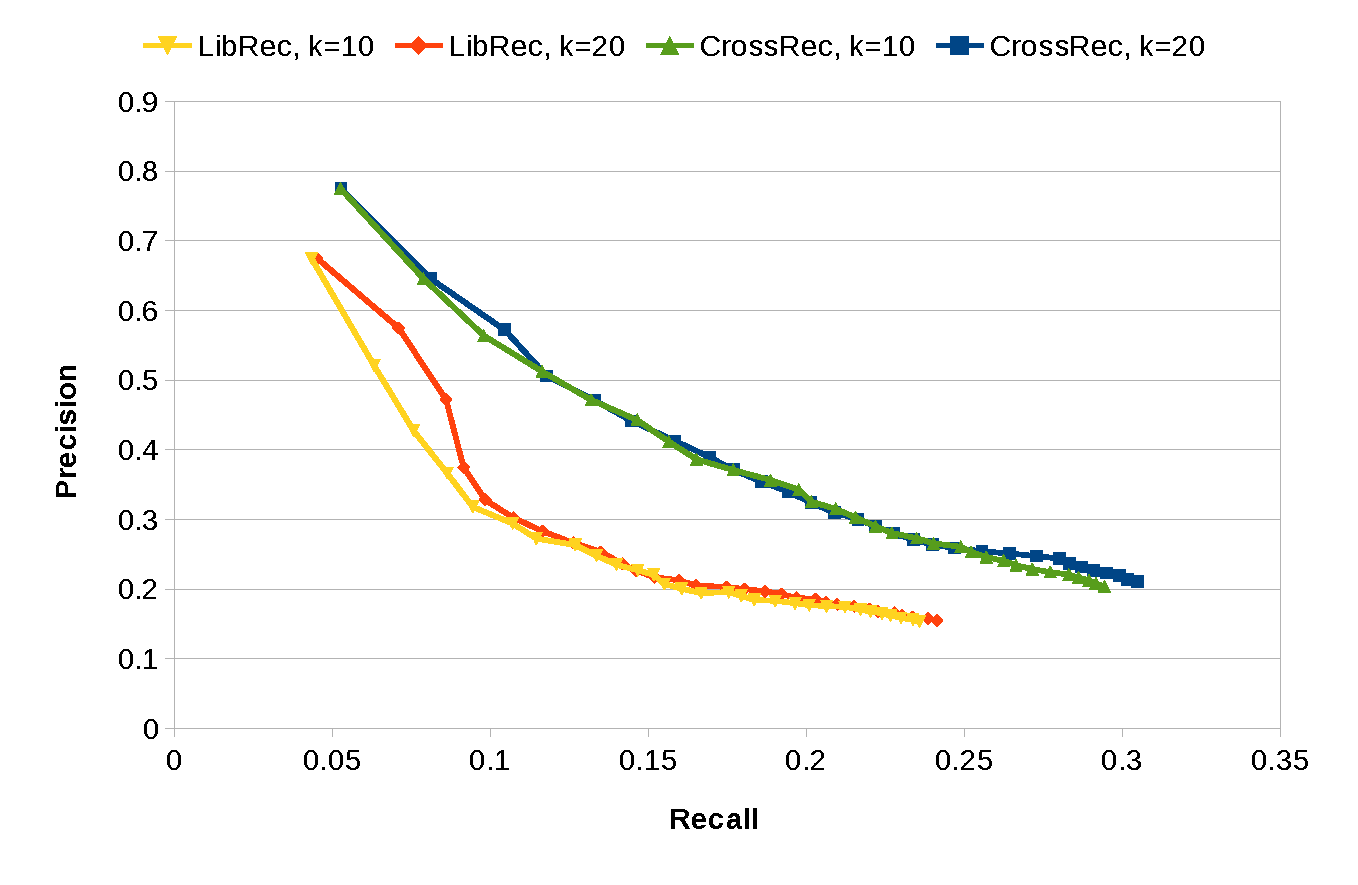
\includegraphics[width=0.45\textwidth]{figs/PrecisionRecall_Fold5.pdf}} & 	
%%		\subfigure[Fold 6]{\label{fig:PrecisionRecallFold6}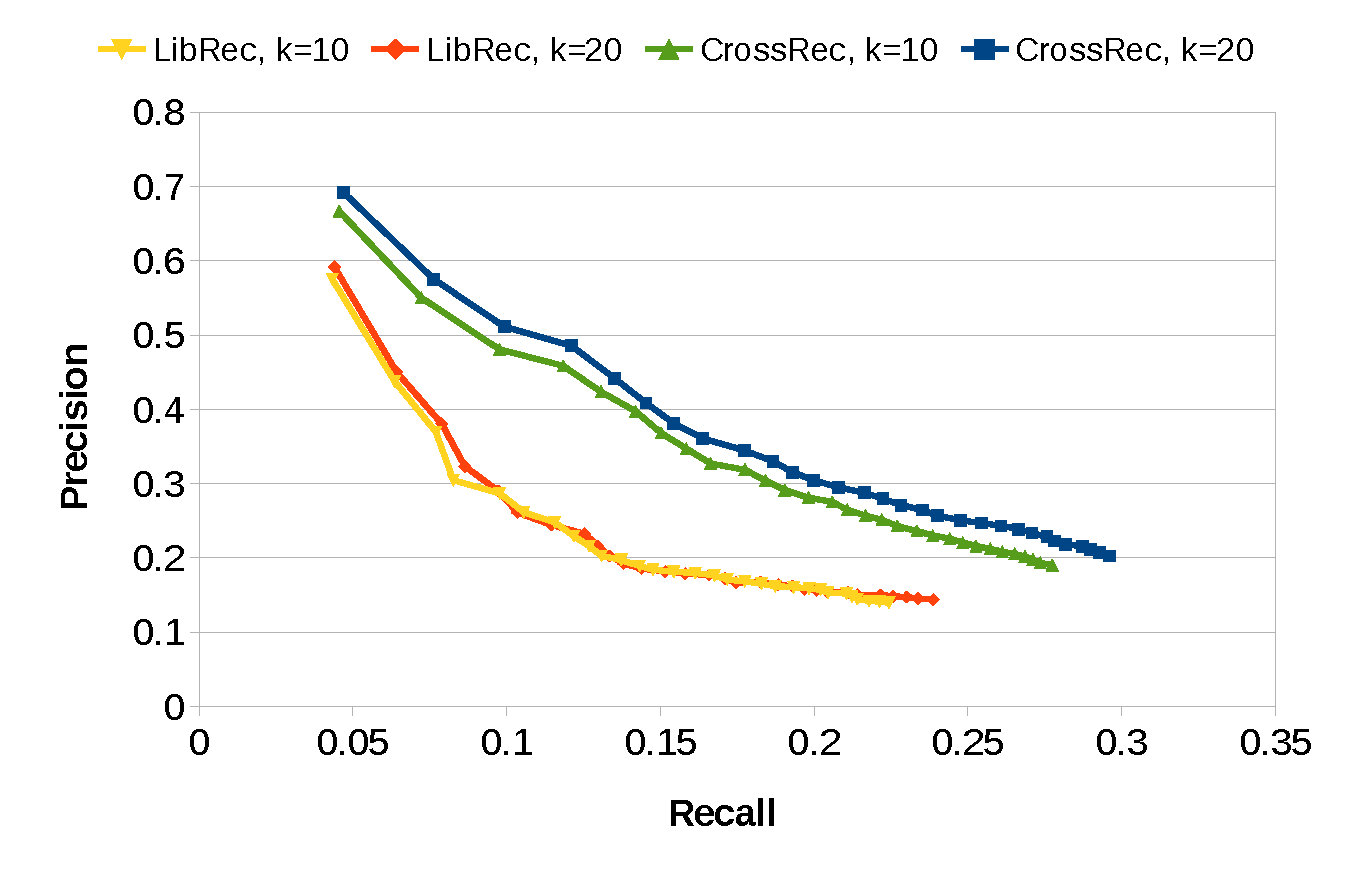
\includegraphics[width=0.45\textwidth]{figs/PrecisionRecall_Fold6.pdf}} \\
%%		\vspace{-.37cm}
%%		\subfigure[Fold 7]{\label{fig:PrecisionRecallFold7}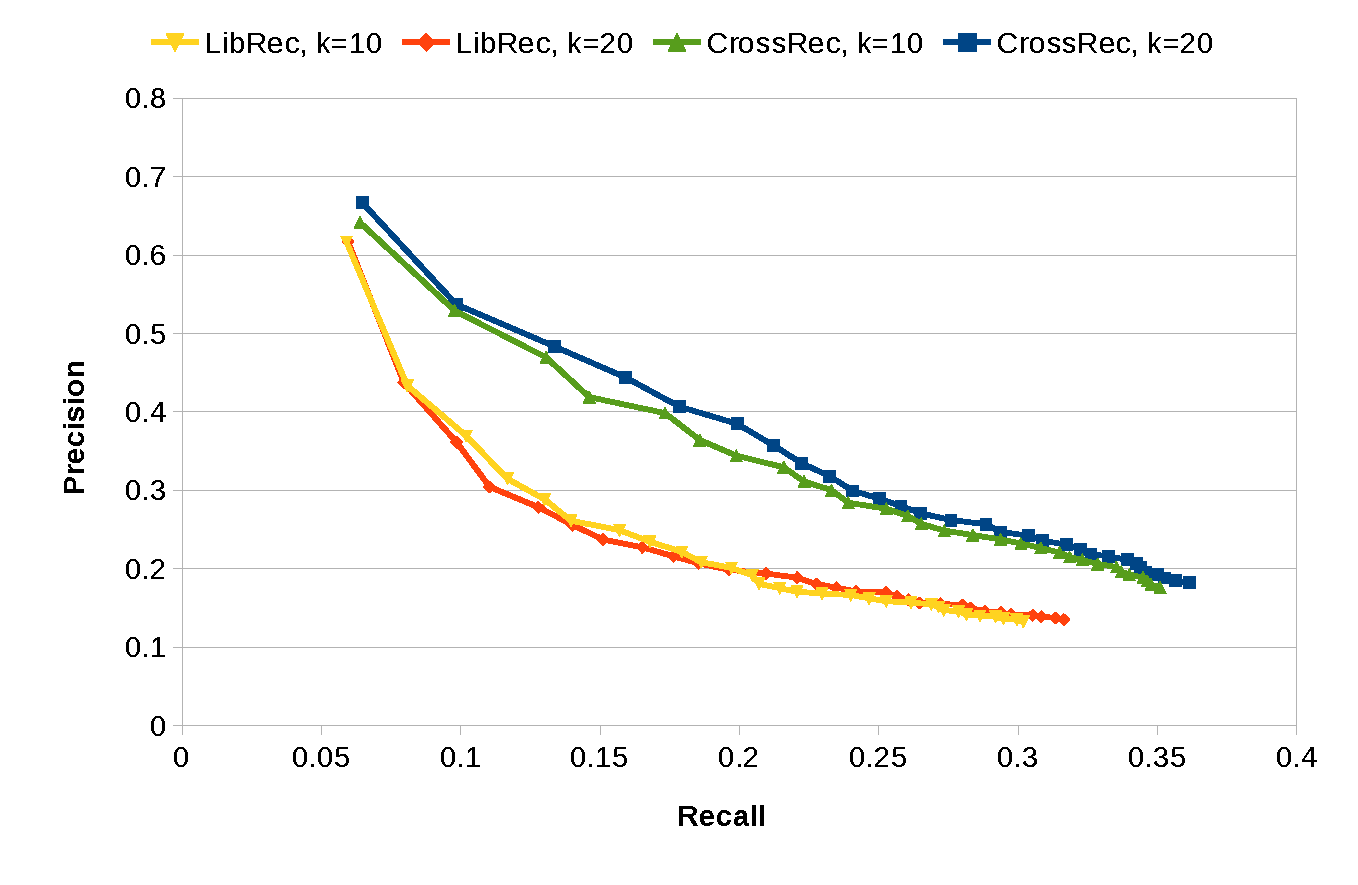
\includegraphics[width=0.45\textwidth]{figs/PrecisionRecall_Fold7.pdf}} & 	
%%		\subfigure[Fold 8]{\label{fig:PrecisionRecallFold8}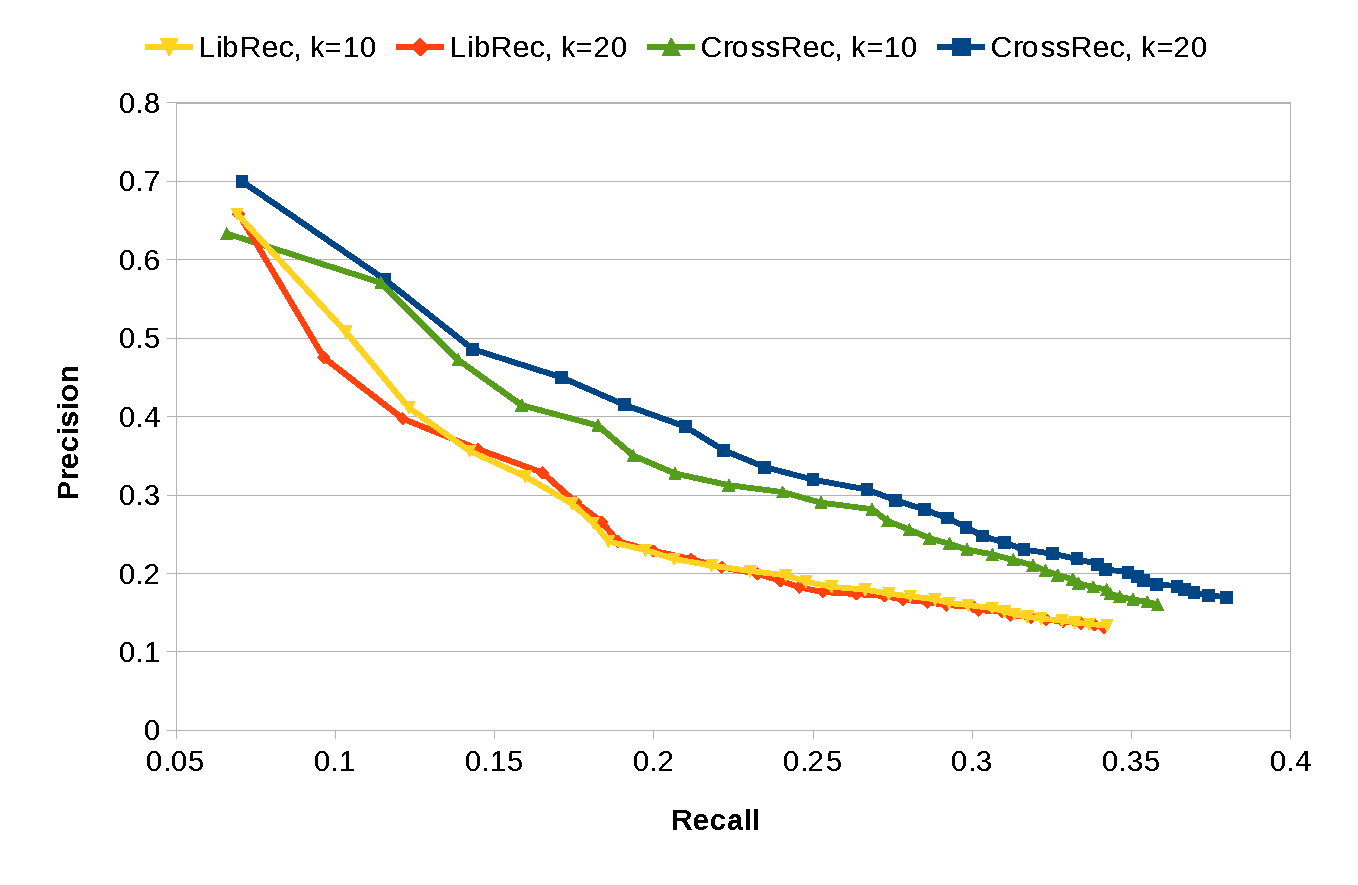
\includegraphics[width=0.45\textwidth]{figs/PrecisionRecall_Fold8.pdf}} \\
%%		\vspace{-.37cm}
%%		\subfigure[Fold 9]{\label{fig:PrecisionRecallFold9}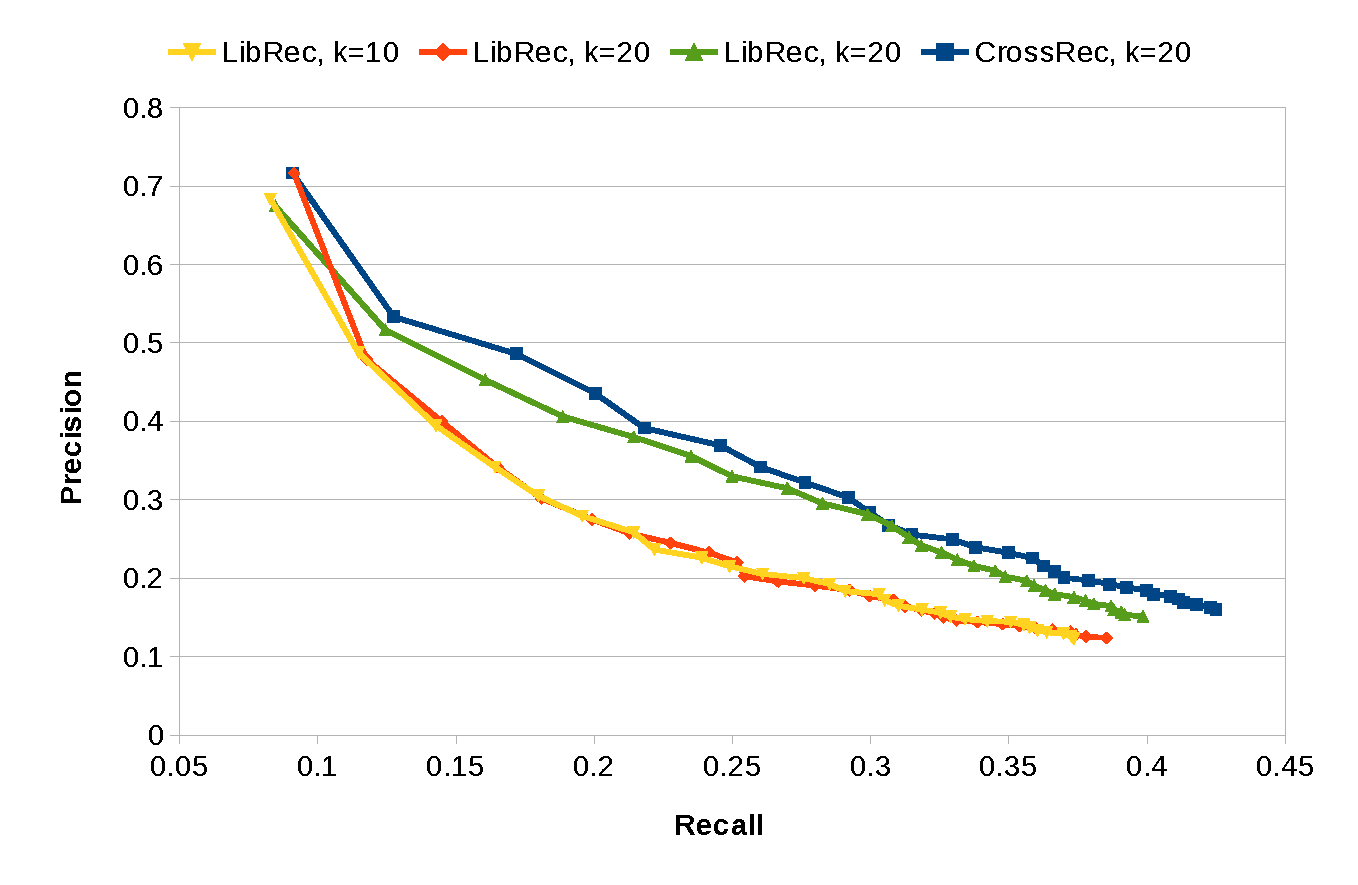
\includegraphics[width=0.45\textwidth]{figs/PrecisionRecall_Fold9.pdf}} & 	
%%		\subfigure[Fold 10]{\label{fig:PrecisionRecallFold10}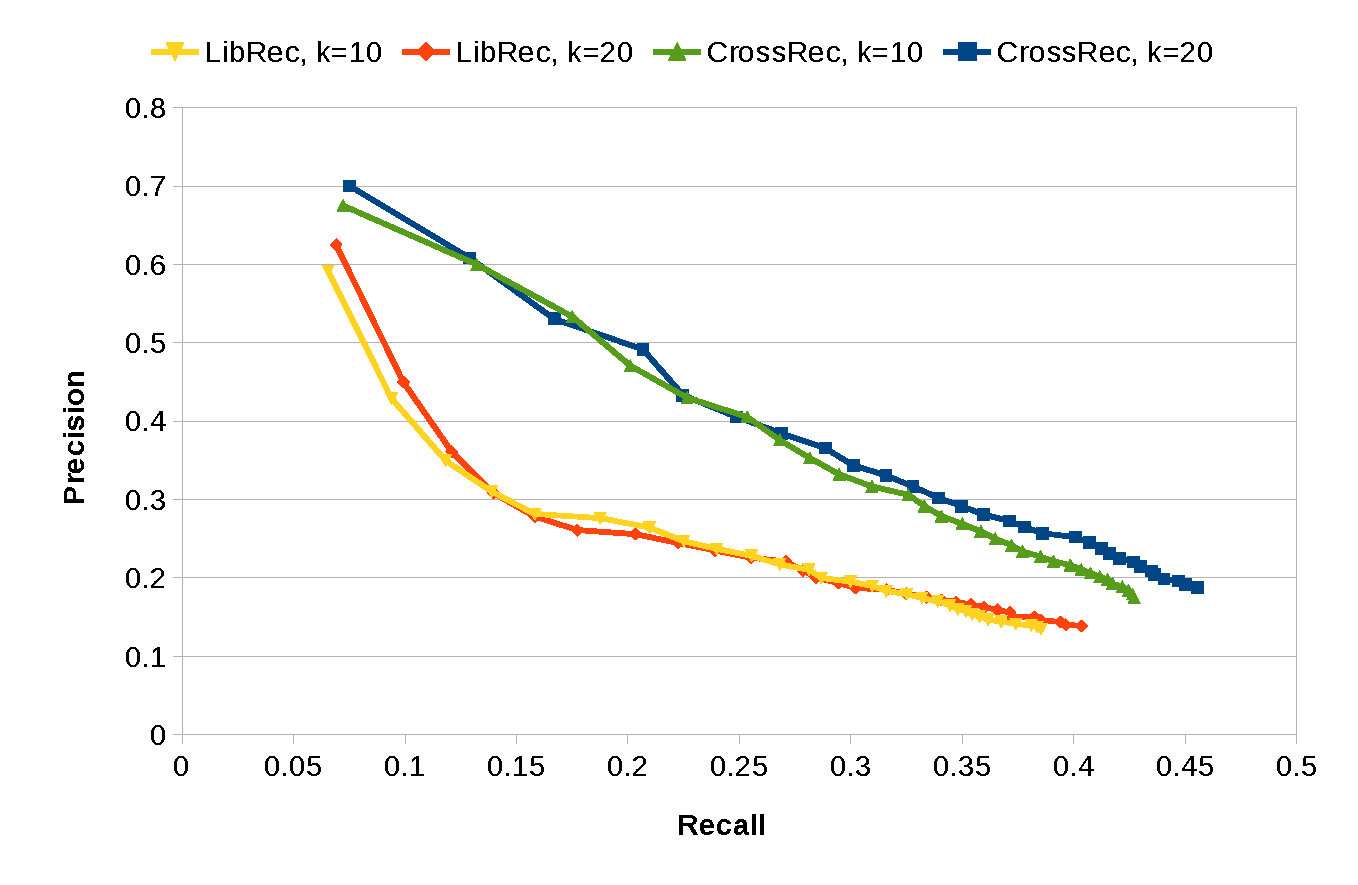
\includegraphics[width=0.45\textwidth]{figs/PrecisionRecall_Fold10.pdf}} \\	
%%	\end{tabular}
%%	\label{fig:PrecisionRecall}	
%%	\caption{\emph{Accuracy: precision@N and recall@N, k=\{10,20\}}}% for \LR and \CR
%%%	\vspace{-.4cm}
%%\end{figure*}
%
%
%
%
%%\vspace{.1cm}
%%%\noindent\textbf{RQ$_1$:} \emph{Does \CR obtain a better success rate compared to \LR?}
%%\noindent \rqsecond
%%\vspace{-.05cm}
%
%
%%
%%\vspace{.1cm}
%%\noindent \revised{\rqsecond}
%%\vspace{-.05cm}
%%
%
%%\begin{table*}[ht]
%%	\footnotesize
%%	\caption{Success rate of \CR on D2 with different number of libraries ($L$).}
%%	\centering
%%%	\begin{tabular}{|r|r|r|r|r|r|r|}\hline
%%	\begin{tabular}{|p{0.7cm}|p{0.7cm}|p{1.0cm}|p{1.0cm}|p{1.0cm}|p{1.0cm}|p{1.0cm}|}\hline
%%		\rowcolor{verylightgray}
%%		\multicolumn{2}{|c|}{} & \multicolumn{5}{c|}{\textbf{Cut-off value (N)}}         \\ \hline%\cline{3-8}
%%%		\rowcolor{verylightgray}
%%		\multicolumn{2}{|c|}{\textbf{Number of libs.}} & 1	 & 3   & 5    & 7   & 10          \\ \hline
%%		{\multirow{2}{*}{$L$}} & 4          & 0.208 & 0.308 & 0.357 & 0.389 & 0.422   \\ \cline{2-7}
%%		& 10         & 0.255 & 0.368 & 0.422 & 0.456 & 0.494   \\ \hline
%%	\end{tabular}
%%	\label{tab:SuccessRate\CRD2}
%%	%\vspace{-.1cm}
%%\end{table*}
%
%\color{black}
%
%
%
%\vspace{.1cm}
%%\textbf{RQ$_2$:} \emph{How well can \LR and \CR recommend third-party libraries in terms of accuracy, sales diversity, and novelty?}
%\noindent \rqsecond
%\vspace{-.05cm}
%
%
%
%
%% $\div$ \ref{fig:PrecisionRecallFold10}
%% \cite{Nguyen:2015:CRV:2942298.2942305}
%
%
%%\LR is highly related to \CR. , we are able to perform a comprehensive evaluation with \LR
%%. 
%%we have access to the source implementation of \LR, thus 
%
%
%
%
%
%
%\noindent%N (the cut-off value for the list of items to be recommended) 
%%\emph{Accuracy:} 
%%We ran both \LR and \CR on \code{D1}. 
%
%\paragraph{\textbf{Accuracy}} To represent accuracy, we vary $N$ from $1$ to $30$ to get \emph{precision@N} and \emph{recall@N}. The rationale behind the selection of $30$ as the maximum cut-off value is that \LR normally produces a short list of recommendations, ranging from $32$ to $50$ items. From the accuracy scores computed using Eq.~\eqref{eqn:Precision} and Eq.~\eqref{eqn:Recall}, the Precision-Recall curves (PRCs) for all $10$ rounds of validation and different values of $k$ were sketched. However, we noticed that the figures representing the folds share a very similar pattern.  Thus, for the sake of clarity, we only show in Fig. \ref{fig:PrecisionRecall} results of the most representative fold. Since a PRC close to the upper right corner represents a better accuracy \cite{DiNoia:2012:LOD:2362499.2362501}, we see that by \LR, changing the number of neighbor $k$ almost makes no difference in its accuracy. Meanwhile for \CR we can notice that an increase of $k$ brings a slightly better accuracy for some testing folds, however the gain is negligible. For all pieces of testing data, \CR always produces a superior accuracy compared to that of \LR.%compared to \LR. %substantially
%
%\begin{figure}[h!]
%	\centering
%	\vspace{-.4cm}
%	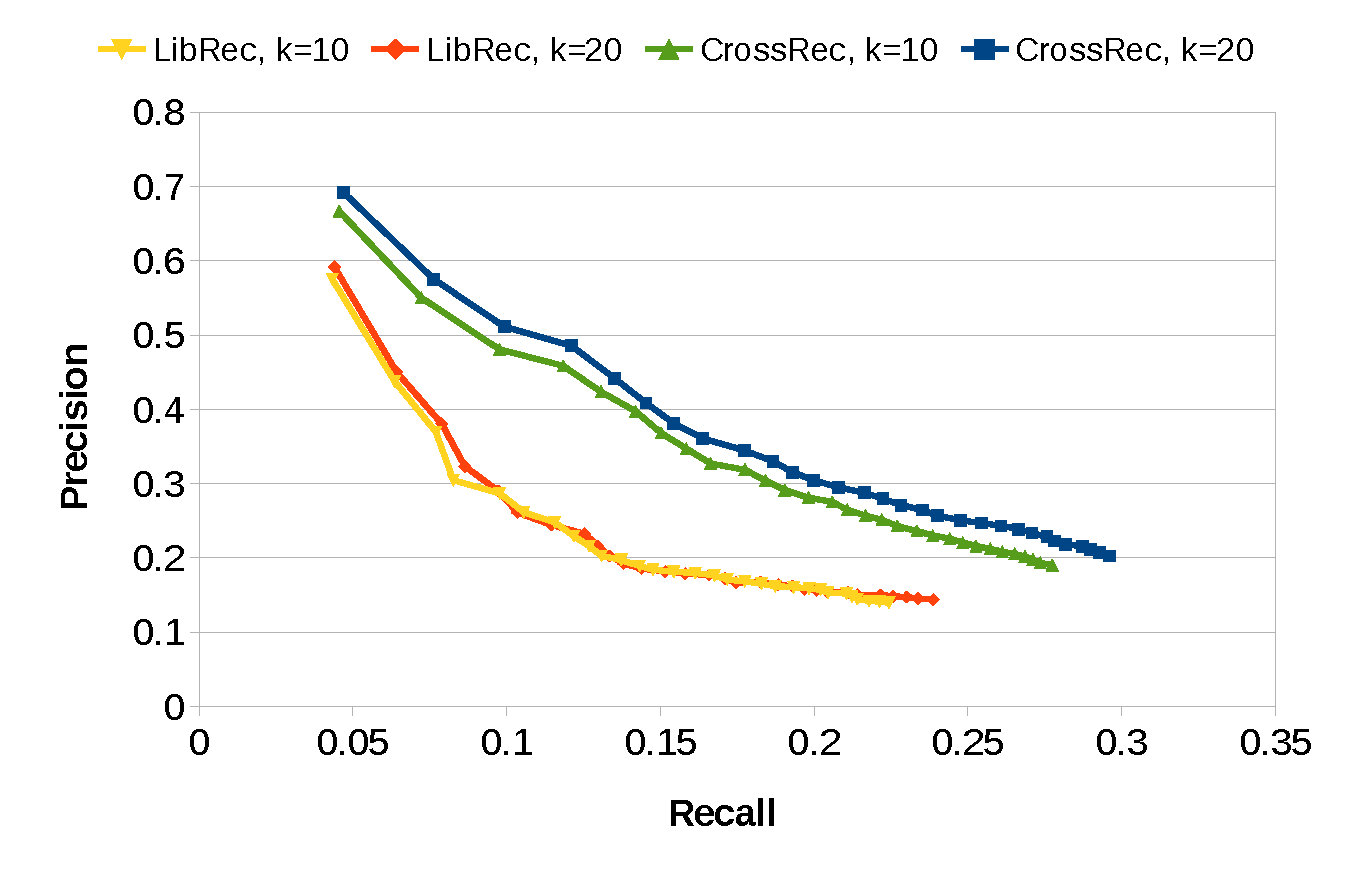
\includegraphics[width=0.86\linewidth]{figs/PrecisionRecall_Fold6.pdf}
%	\vspace{-.7cm}
%	\caption{Precision and Recall.}
%	\label{fig:PrecisionRecall}
%	\vspace{-.5cm}
%\end{figure}
%
%
%
%
%
%
%%\begin{tcolorbox}[boxrule=0.86pt,left=0.3em, right=0.3em,top=0.1em, bottom=0.05em]
%%	\small{In summary, we see that \CR significantly outperforms \LR 
%%		in all considered test configurations concerning \emph{success rate}, with 
%%		a large effect size. The recommendation time for a fold (120 projects) is 
%%		relatively faster for \CR (3s) than for \LR (20s).}
%%\end{tcolorbox}
%
%
%
%
%
%\vspace{.1cm}
%\noindent
%%\emph{Sales Diversity:} 
%\paragraph{\textbf{Sales diversity}} The catalog coverage scores for \LR and \CR are depicted in Table 
%\ref{tab:CatalogCoverage}. The maximum coverage values are $4.594$ and $5.897$ for \LR and 
%\CR, respectively. According to Eq. \eqref{eqn:Coverage}, a higher score means a better 
%coverage. In this sense, the recommendations generated by \CR cover a wider spectrum of 
%libraries than those by \LR for both configurations, \ie $k=10$ and $k=20$, using different 
%cut-off values $N$. Table \ref{tab:Entropy} shows the \emph{entropy} for \LR and \CR. 
%Equation \eqref{eqn:Entropy} suggests that a low entropy value represents a better distribution of 
%items, therefore the recommendations by \CR have a much better distribution than those 
%obtained by \LR. For example, for the case $N=25$ and $k=20$, \CR has an entropy of $0.635$, 
%which is much better than $2.751$, the corresponding value by \LR.
%
%\begin{table}[h!]
%	\footnotesize
%	\caption{Catalog coverage for N=\{5,10,15,20,25\}, k=\{10,20\}.}
%	\centering
%	\begin{tabular}{|p{0.8cm}||p{1.2cm}|p{1.2cm}||p{1.2cm}|p{1.2cm}|} \hline	
%%		\rowcolor{verylightgray}	
%		& \multicolumn{2}{c||}{\textbf{k=10}}  & \multicolumn{2}{c|}{\textbf{k=20}} \\ \hline
%		\textbf{N}	& \LR    & \CR  & \LR    & \CR	  \\ \hline	
%		5       & 0.857   	  & \textbf{1.099}  	& 0.691 		& \textbf{0.814}    \\ \hline
%		10      & 1.760      & \textbf{2.157}  	& 1.346 		& \textbf{1.534}    \\ \hline
%		15      & 2.675      & \textbf{3.278}  	& 1.937 		& \textbf{2.312}    \\ \hline
%		20      & 3.577      & \textbf{4.541}  	& 2.512 		& \textbf{3.143}    \\ \hline
%		25      & 4.594      & \textbf{5.897}  	& 3.139 		& \textbf{4.005}    \\ \hline
%	\end{tabular}
%	\label{tab:CatalogCoverage}
%\end{table}
%
%%According to Table \ref{tab:CatalogCoverage}, increasing the number of neighbours for recommendation adds a decline in coverage for both systems. %Referring to 
%% by this quality indicator, surpasses \LR in the recommendation performance. %gains a better performance compared to that of \LR. 
%% by this quality indicator, 
%
%\begin{table}[h!]
%	\footnotesize
%	\caption{Entropy for N=\{5,10,15,20,25\}, k=\{10,20\}.}
%	\centering
%	\begin{tabular}{|p{0.8cm}||p{1.2cm}|p{1.2cm}||p{1.2cm}|p{1.2cm}|} \hline		
%%		\rowcolor{verylightgray}
%		& \multicolumn{2}{c||}{\textbf{k=10}}  & \multicolumn{2}{c|}{\textbf{k=20}} \\ \hline
%		\textbf{N}	& \LR    & \CR  & \LR    & \CR	  \\ \hline	
%		5       & 0.869   	 & \textbf{0.239}  	& 0.552 		& \textbf{0.127}    \\ \hline
%		10      & 1.752      & \textbf{0.481}  	& 1.098 		& \textbf{0.254}    \\ \hline
%		15      & 2.653      & \textbf{0.723}  	& 1.639 		& \textbf{0.381}    \\ \hline
%		20      & 3.566      & \textbf{0.968}  	& 2.193 		& \textbf{0.508}    \\ \hline
%		25      & 4.500      & \textbf{1.217}  	& 2.751 		& \textbf{0.635}    \\ \hline
%	\end{tabular}
%	\vspace{-.1cm}
%	\label{tab:Entropy}
%\end{table}
%
%
%\noindent
%%\emph{Novelty:} 
%\paragraph{\textbf{Novelty}} The \emph{EPC@N} scores for \LR and \CR are shown in Table~\ref{tab:EPC}. With \LR, changing $k$ from $10$ to $20$ decreases \emph{novelty} for all cut-off values. For example, the \emph{novelty} with $N=25$ and $k=10$ is $0.349$, however once $k$ is changed to $20$, it drops to $0.261$. For \CR, changing the number of neighbours \emph{k} from $10$ to $20$ does not bring a rise in \emph{novelty}. As shown in Table~\ref{tab:EPC}, \CR always obtains scores that are higher than those of \LR. For example, when $N=5$ and $k=20$, \CR achieves a value of $0.292$ for \emph{novelty}, whereas \LR gets $0.114$. This, together with the example in Section~\ref{sec:Example}, confirms that \CR recommends libraries that are closer to the long tail than \LR can do.  %with respect to \emph{Novelty} 
%%\vspace{-.2cm}
%
%\begin{table}[t]
%	\footnotesize
%	\caption{EPC for N=\{5,10,15,20,25\}, k=\{10,20\}.}
%	\centering
%	\begin{tabular}{|p{0.8cm}||p{1.2cm}|p{1.2cm}||p{1.2cm}|p{1.2cm}|} \hline	
%%		\rowcolor{gray}	
%		& \multicolumn{2}{c||}{\textbf{k=10}}  & \multicolumn{2}{c|}{\textbf{k=20}} \\ \hline
%		\textbf{N}	& \LR    & \CR  & \LR    & \CR	  \\ \hline	
%		5       & 0.187	   	 & \textbf{0.291}  	& 0.114	 		& \textbf{0.292}    \\ \hline
%		10      & 0.264      & \textbf{0.349}  	& 0.166  		& \textbf{0.344}    \\ \hline
%		15      & 0.296      & \textbf{0.376}  	& 0.204 		& \textbf{0.377}    \\ \hline
%		20      & 0.320      & \textbf{0.391}  	& 0.236 		& \textbf{0.399}    \\ \hline
%		25      & 0.349      & \textbf{0.401}  	& 0.261 		& \textbf{0.416}    \\ \hline
%	\end{tabular}
%	\label{tab:EPC}
%\end{table}
%
%
%
%\begin{table*}[h!]
%	\footnotesize
%	\caption{Wilcoxon rank sum test adjusted $p$-values for N=\{3,5,10,15\}, 
%		k=10.}
%	\centering
%	\begin{tabular}{|p{0.8cm}||p{1.2cm}|p{1.2cm}||p{1.2cm}|p{1.2cm}||p{1.2cm}|} \hline	
%		%	\begin{tabular}{|r||r|r||r|r||r|}\hline
%%		\rowcolor{gray}
%		& \multicolumn{2}{c||}{\textbf{Accuracy}} &  \multicolumn{2}{c||}{\textbf{Sales Diversity}}   & \textbf{Novelty}  \\ \hline
%		\textbf{N} & Precision  &  Recall   & Coverage   & 	Entropy  & EPC \\\hline
%		3          & 1.58e-16&5.41e-08 & 0.0005 & 6.50e-05& 4.33e-05 \\\hline
%		5          & 1.35e-24& 9.10e-12 & 0.001 & 6.50e-05& 4.33e-05 \\\hline
%		10         & 1.07e-21& 9.12e-12 & 0.003& 4.33e-05& 1.52e-04 \\\hline
%		15         &  1.10e-14 & -- & 0.003& 6.50e-05& 2.06e-04 \\\hline
%	\end{tabular}
%	\label{tab:Wilcoxon}
%\end{table*}
%%
%
%
%\begin{table*}[h!]
%	\footnotesize
%	\caption{Cliff's $d$ results for N=\{3,5,10,15\}, k=10. Labels in parenthesis indicate the magnitude (n:negligible, s:small, l:large).}
%	\centering
%	\begin{tabular}{|p{0.8cm}||p{1.2cm}|p{1.2cm}||p{1.2cm}|p{1.2cm}||p{1.2cm}|} \hline	
%		%	\begin{tabular}{|r||r|r||r|r||r|}\hline
%%		\rowcolor{gray}
%		& \multicolumn{2}{c||}{\textbf{Accuracy}} &  \multicolumn{2}{c||}{\textbf{Sales Diversity}}   & \textbf{Novelty}  \\ \hline
%		\textbf{N} & Precision & Recall  & Coverage & Entropy & EPC  \\ \hline
%		3          &  0.18 (s) & 0.12 (n)& 0.92 (l)& 0.96 (l)& 1.00 (l) \\ \hline
%		5          &  0.23 (s) & 0.16 (s)& 0.86 (l)&  0.98 (l)& 1.00 (l) \\ \hline
%		10         &  0.22 (s) & 0.16 (s)& 0.80 (l)&  1.00 (l)& 0.94 (l) \\ \hline
%		15         &  0.17 (s) & -- & 0.80 (l)&  0.98 (l) & 0.90 (l)\\ \hline
%	\end{tabular}
%	\label{tab:Cliff}
%	%\vspace{-.1cm}
%\end{table*}
%
%
%
%%====================old tables are here========================================
%%===============================================================================
%%\begin{table*}[h!]
%%	\footnotesize
%%	\caption{Wilcoxon rank sum test adjusted $p$-values for N=\{3,5,10,15\}, 
%%		k=10.}
%%	\centering
%%	\begin{tabular}{|r|r|r|r|r|r|r|}
%%		\hline
%%		\rowcolor{verylightgray}
%%		& \textbf{Success Rate} &     
%%		\multicolumn{2}{c|}{\textbf{Accuracy}}      &   
%%		\multicolumn{2}{c|}{\textbf{Sales Diversity}}   & \textbf{Novelty}      
%%		\\ \hline
%%		\textbf{N} & Success Rate          & Precision               & 
%%		Recall                & Coverage                  & 
%%		Entropy               & EPC                   \\ \hline
%%		3          & 0.02& 1.58e-16&5.41e-08 & 0.0005 & 6.50e-05& 4.33e-05\\ 
%%		\hline
%%		5          & 0.02& 1.35e-24& 9.10e-12 & 0.001 & 6.50e-05& 4.33e-05\\ 
%%		\hline
%%		10          & 0.17& 1.07e-21& 9.12e-12 & 0.003& 4.33e-05& 1.52e-04\\ 
%%		\hline
%%		15          & 0.002&  1.10e-14 & -- & 0.003& 6.50e-05& 2.06e-04\\ \hline
%%	\end{tabular}
%%	\label{tab:Wilcoxon}
%%\end{table*}
%%%
%%\begin{table*}[ht]
%%	\footnotesize
%%	\caption{Cliff's $d$ results for N=\{3,5,10,15\}, k=10. Labels in parenthesis indicate the magnitude (n:negligible, s:small, l:large).}
%%	\centering
%%	\begin{tabular}{|r|r|r|r|r|r|r|}\hline
%%		\rowcolor{verylightgray}
%%		& \textbf{Success Rate} &     \multicolumn{2}{c|}{\textbf{Accuracy}}      &   \multicolumn{2}{c|}{\textbf{Sales Diversity}}   & \textbf{Novelty}      \\ \hline
%%		\textbf{N} & Success Rate          & Precision               & Recall                & Coverage                  & Entropy               & EPC                   \\ \hline
%%		3          & 0.70 (l)& 0.18 (s)& 0.12 (n)& 0.92 (l)& 0.96 (l)& 1.00 (l) \\ \hline
%%		5          & 0.74 (l)&  0.23 (s)& 0.16 (s)& 0.86 (l)&  0.98 (l)& 1.00 (l) \\ \hline
%%		10         & 0.93 (l)&  0.22 (s)& 0.16 (s)& 0.80 (l)&  1.00 (l)& 0.94 (l) \\ \hline
%%		15         & 0.58 (l)&  0.17 (s)& -- & 0.80 (l)&  0.98 (l) & 0.90 (l)\\ \hline
%%	\end{tabular}
%%	\label{tab:Cliff}
%%	%\vspace{-.1cm}
%%\end{table*}
%%===============================================================================
%
%
%
%Also in this case (see columns 2-6 of Tables \ref{tab:Wilcoxon} and \ref{tab:Cliff}), our analyses are supported by statistical procedures. Differences are always statistically significant. The effect size is negligible/small for \emph{accuracy} (precision and recall), whereas it is large for all other indicators \emph{sales diversity} and \emph{novelty}.
%
%
%
%\begin{tcolorbox}[boxrule=0.86pt,left=0.3em, right=0.3em,top=0.1em, bottom=0.05em]
%	\small{The results in Fig.~\ref{fig:PrecisionRecall} and 
%		Tables~\ref{tab:CatalogCoverage},~\ref{tab:Entropy},~\ref{tab:EPC} demonstrate 
%		that \CR significantly outperforms \LR concerning 
%		\emph{accuracy}, \emph{sales diversity}, and \emph{novelty}, with a 
%		small/negligible effect size for \emph{accuracy} and large elsewhere.}
%\end{tcolorbox}
%
%%. Furthermore, \CR significantly outperforms 
%
%%\begin{tcolorbox}[boxrule=0.86pt,left=0.3em, right=0.3em,top=0.1em, bottom=0.05em]
%%%	\color{blue}
%%	\revised{\small{%The results in Fig.~\ref{fig:PrecisionRecall} and Tables~\ref{tab:CatalogCoverage},~\ref{tab:Entropy},~\ref{tab:EPC} 	
%%	Altogether, we see that \CR significantly outperforms \LR in all considered test configurations concerning \emph{success rate}, with a large effect size, and concerning \emph{accuracy}, \emph{sales diversity}, and \emph{novelty}, with a small/negligible effect size for \emph{accuracy} and large elsewhere. The recommendation time for a fold (120 projects) is relatively faster for \CR (3s) than for \LR (20s).}}
%%	\color{black}
%%\end{tcolorbox}
%
%
%
%%\vspace{.2cm}
%%\textbf{RQ$_3$:} \emph{Is the performance difference between the two systems statistically significant?}
%%\vspace{.1cm}
%%
%%To see if the improvement of the proposed approach is statistically significant and substantial, we perform a Wilcoxon rank sum test \cite{Wilcoxon1992} on all the quality scores for both systems, using $k=10$ and $N=\{3,5,10,15\}$. The $p$-values for all quality metrics are shown in Table~\ref{tab:Wilcoxon}. The null hypothesis is that there are no differences between the performance of \CR and that of \LR. Using $5\%$ as the confidence level, we see that by all quality indicators the \emph{p-values} are always lower than $5 \times e^{-2}$. Cliff's $d$ values are reported in Table \ref{tab:Cliff}. As the table shows, the observed differences are always in favor of \CR (\ie effect sizes are always positive). Magnitude of the computed Cliff's $d$ is small for precision and recall, while it is large for all other indicators, including Success Rate.
%%
%%\begin{tcolorbox}
%%In this sense, we reject the null hypothesis and conclude that the performance improvement obtained by \CR is statistically significant. %or \emph{p-value} $< 5 \times e^{-2}$ . in terms of all quality metrics. 
%%\end{tcolorbox}
%
%\vspace{.1cm}
%%\textbf{RQ$_3$:} \emph{What are the reasons for the performance difference?}
%\noindent \rqthird
%\vspace{-.05cm}
%
%%Last but not least, w
%%\PN{The explanation has been substantially improved compared to the old version}
%We attempt to ascertain why \CR outperforms \LR. This task might necessitate further investigations, both 
%qualitative and quantitative research. However, by carefully studying the internal design of \LR, we found out that 
%the improvement attributes to the following facts. In the first place, \CR employs a completely different approach 
%to represent projects and libraries: it encodes the relationships among them into a graph. Second, to compute the 
%similarity between two projects, \CR assigns a weight to every library node using tf-idf (see 
%Eq.~\eqref{eqn:TFIDF}). In this way, the level of importance of a node is disproportional to its popularity. This is 
%similar to the context of document matching where popular terms are given a low weight 
%\cite{DBLP:journals/ijswis/HliaoutakisVVPM06}. For instance, in Fig.~\ref{fig:Graph}, $lib_1$ is a popular node since 
%it is referred by $4$ projects and this makes it have a low weight. As a result, \CR is able to better capture the 
%similarity between two projects compared to \LR, which equally treats all libraries. Third, \LR employs a very 
%simple collaborative-filtering technique, though it also considers a set of k-nearest neighbor similar projects for 
%finding libraries, it neglects their similarity level by considering all projects in the same way.~Also, the technique 
%assigns more weight to popular libraries without considering the degree of similarity between projects, from where the 
%libraries come. This explains why \LR recommends very popular items as shown in Section~\ref{sec:Example}.~In 
%contrast, \CR improves by assigning a larger weight to libraries that come from highly similar projects (see 
%Eq.~\eqref{eqn:Prediction}). In other words, given a project, \CR is able to ``mimic'' the behavior of highly 
%similar projects, it attempts to suggest a comparable set of libraries. Lastly, \LR exploits association rule mining 
%which indeed mines items that co-exist. This is why the coverage of the recommended items is low compared to what 
%achieved by \CR.
%
%\begin{tcolorbox}[boxrule=0.86pt,left=0.3em, right=0.3em,top=0.1em, bottom=0.05em]
%	\small{Our qualitative analysis suggests that the improvements achieved by 
%		\CR with respect to \LR are due to the weighting scheme being 
%		applied, which also considers the projects' similarity, \ie it rewards 
%		recommendation of libraries from similar projects.}
%	%Altogether, we see that the improvement by \CR is obtained thanks to the weighting scheme applied to both libraries and projects. With \CR, the collaborative-filtering technique is well practiced in the sense that highly similar projects are more preferred to be mined. Meanwhile, \LR employs a na\"ive collaborative-filtering technique, which ignores the degree of similarities among projects by treating them equally. As a result, the libraries recommended by \CR are more relevant, even though they are not popular. %Furthermore, since \LR prefers high frequency libraries, which decreases novelty. 
%\end{tcolorbox}
%%\vspace{-.2cm}
%
%%The association rule mining module also contributes to 
%
%
%
%
%%\color{blue}
%
%\vspace{.1cm}
%\noindent \revised{\rqfourth}
%\vspace{-.05cm}
%
%
%%amount of data used as query. ratio of 
%% as the ratio of query to testing data
%\revised{Finally, we studied whether an increase in the input data contributes to an improvement in the performance of \CR. As it was already mentioned in Section~\ref{sec:ResearchQuestions}, $r$ is the ratio of libraries used as query over the total number of libraries that a project contains. For this evaluation, rather than using $r=50\%$, we varied it along the following values: $20\%$, $40\%$, $60\%$, and $80\%$, and measured the achieved level of performance. This simulates different levels of a project's maturity: at the beginning when the developer has just included a small number of libraries, or later on when more libraries have been accumulatively populated alongside the project's lifecycle. This research question aims at studying if \CR can assist the developer in choosing the right libraries at different stages of the development process.}
%
%
%\begin{figure}[h!]
%	%	\color{blue}
%	\centering
%	%	\vspace{-.4cm}
%	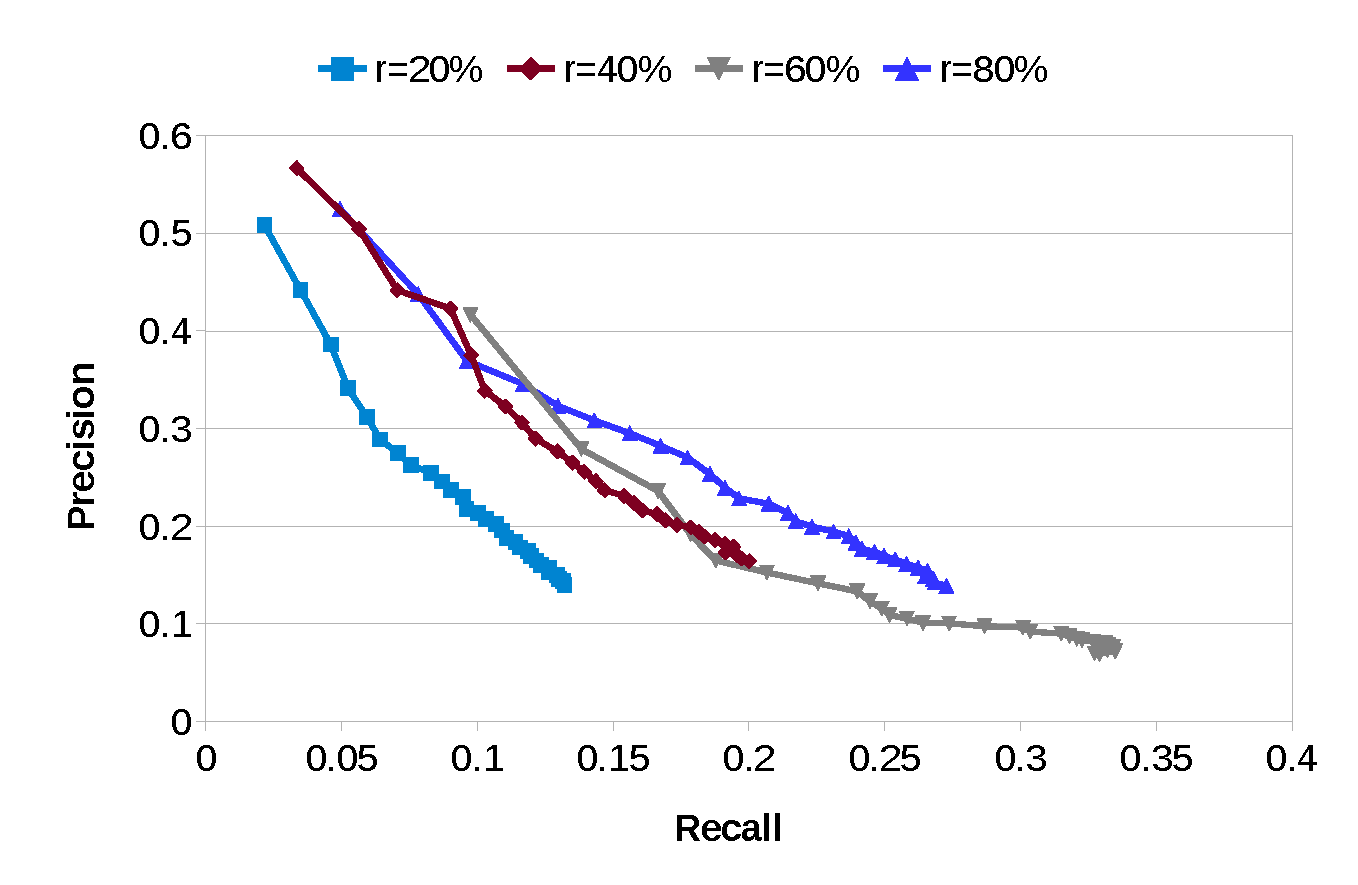
\includegraphics[width=0.86\linewidth]{figs/PrecisionRecall_QueryGroundTruth.pdf}
%	%	\vspace{-.7cm}
%	\caption{\revised{Precision and recall for different amounts of testing and ground-truth data.}}
%	\label{fig:PrecisionRecall_QueryGroundTruth}
%	%	\vspace{-.5cm}
%\end{figure}
%
%%As a PRC close to the upper right corner corresponds to 
%%However, the tendency tends to stagnate when $r$ becomes larger. 
%
%\revised{Fig.~\ref{fig:PrecisionRecall_QueryGroundTruth} reports the precision and recall curves (PRCs) obtained by the configurations. As a better accuracy is represented by a PRC close to the upper right corner~\cite{DiNoia:2012:LOD:2362499.2362501},\cite{Davis:2006:RPR:1143844.1143874}, we see that generally there is an improvement in the recommendation performance when $r$ increases. In particular, there is a sharp growth in precision and recall when $r$ is changed from $20\%$ to $40\%$. However, the gain tends to stagnate when $r$ becomes larger. For instance, the change in performance between $r=40\%$ and $r=60\%$ is small and can be considered as negligible. Similarly, when $r$ goes up to $80\%$ from $60\%$, there is also a marginal change in accuracy. This corresponds to a saturation: at a certain threshold of $r$, \eg $r=50\%$ or $r=60\%$, a little or almost no performance gain can be obtained. In essence, that means \CR can achieve a decent level of accuracy once the developer has included around a half of the total number of libraries.}
%
%
%
%\begin{tcolorbox}[boxrule=0.86pt,left=0.3em, right=0.3em] %,top=0.1em, bottom=0.05em
%	%	\color{blue}
%	\revised{\small{For \CR, an increase in the amount of input data considerably improves the overall performance when the ratio of query to testing data $r$ is small. However, such the gain is disproportionate to $r$.}}
%\end{tcolorbox}
%
%\color{black}
%
%
%\subsection{Threats to Validity} \label{sec:ThreatsToValidity}
%
%We identify the threats that may adversely affect the validity of the experiments as well as the countermeasures taken to mitigate them. %In particular, we focus on internal andexternal threats to validity as discussed below.
%
%\noindent\textit{Threats to internal validity}  are related to any factors internal to our study that can influence our results. 
%%In the performed experiments, we did not consider the version number of project libraries. Even though this is a limitation of the current implementation of \CR, also \LR neglects library versions and consequently the performance comparison between the two systems has not been affected.
%The performances achieved by \CR can depend on the values of $N$ and $k$. We showed in the paper results for $k=10, 20$, and for $N=5, 10, 15, 20, 25$ (see more in Section \ref{sec:Discussions}). Results for other values of $N$ and $k$ are consistent with what we already found.
%
%\revised{The comparison with \LF and \LC has been done in an indirect manner through their corresponding datasets, and this might possibly pose a threat to internal validity. We attempted to mitigate such a threat by exploiting the same experimental settings as well as performing various trials on the same datasets. All the additional experiments yielded comparable outcomes to those presented in the paper.}
%
%
%%By the evaluation, besides the main experiments, we conducted additional trials 
%%using various combinations of $N$ and $k$ to further validate the outcomes. All 
%%the additional experiments produced comparable outcomes to those presented in 
%%the paper.
%
%%As we explained in Section \ref{sec:\CR}, \CR recommends libraries and not specific library versions. It is possible that in a specific context a given library version might be more relevant than another, or even than a different library. We plan to investigate with this specific limitation in our future work.
%
%\noindent\textit{Threats to external validity} concern the 
%generalizability of our findings. In the data collection phase, we tried to 
%cover a wide range of possibilities by mitigating also the fact that  many 
%repositories in GitHub are of low quality, which is especially true when they 
%do not have many stars. The set of  $1,200$ GitHub projects was 
%randomly created by obtaining the following distribution of stars: 14 projects 
%have 0 stars, 135 projects have $[$1-4$]$ stars, 66 projects have $[$5-9$]$ 
%stars, 512 projects have $[$10-99$]$ stars, 300 projects have $[$100-499$]$ 
%stars, 78 projects have $[$500-999$]$ stars, and 95 projects have more than 
%1,000 stars. Moreover, the number of libraries that a project in the considered dataset 
%includes varies considerably from $10$ to more than $500$. 
%
%
%%They are related to the experimental settings presented in the paper, concerning the simulated setting used to evaluate the tool. 
%%
%
%\noindent\textit{Threats to construct validity} are whether the setup and measurement in the study reflect real-world 
%situations. The threats have been mitigated by applying ten-fold cross validation, attempting to simulate a real 
%scenario of recommending third-party libraries. In the experiments, the dataset is split into two independent parts, 
%namely a \emph{training set} and a \emph{testing set}. In practice, the items in the training data correspond to the 
%OSS projects collected a priori.~They are available at developers' disposal, ready to be exploited for any mining 
%purpose. Whereas, an item in the testing data corresponds to the project being developed. In this sense, our evaluation 
%attempts to mimic a real deployment: the recommender systems should produce recommendations for a project based on the 
%data available from a set of existing projects.
%
%%
%%as follows. The set of $1,200$ GitHub projects was randomly collected, and the 
%%number of libraries that a project includes varies considerably from $10$ to 
%%more than $500$. 
%%
%% as shown in Fig.~\ref{fig:NumOfPros}
%%In this sense, we can the generalize the study's findings beyond the projects considered in the evaluation.%This implies that our proposed approach can generalize generalizability is preserved. %concerns to the generalizability of the results. 
%%\vspace{-.2cm}
%\subsection{Discussions} \label{sec:Discussions}
%
%%transcend (in lieu of overcome)
%
%%\color{blue}
%
%\revised{\CR is capable of recommending a library (either just the library, or also a specific version of that library), depending on the availability of the training data. That is, the \CR approach transcends the limitation of the baselines considered in this paper, \ie~\LR, \LF and \LC. Such approaches cannot recommend a specific version of a library. Moreover, \CR obtains a better performance when the input data is more dense, \ie more libraries are available for training.}
%
%%\revised{In the first place, \CR overcomes the limitation of all the baselines considered in this paper since it is capable of recommending libraries with versions. Moreover, \CR obtains a better performance when the input data is denser, \ie more libraries are available for training.}
%
%%\color{black}
%
%By performing experiments with \LR and \CR on the same dataset, and by applying the same experimental settings, we were able to compare their performance in a thorough manner. We have seen that an increase in the number of neighbor projects considered for recommendation from $k=10$ to $k=20$ does not make a big distinction in accuracy for both systems. Furthermore, as there are no changes in success rates by increasing $k$, we can conclude that almost all relevant libraries are in the top-most similar projects. This is further enforced by the fact that the \emph{entropy} improves for both systems when $k$ is increased from $10$ to $20$. The inclusion of more projects brings various libraries, and this  helps to increase the item distribution. With \LR, the fact that the \emph{novelty} decreases when $k$ increases shows that the additional projects bring only popular libraries. At the same time, the \emph{novelty} does not change with \CR using the same setting with $k$. This indicates that the recommended libraries brought by the additional projects do not help improve the overall \emph{novelty}.  
%
%In this sense, the ability to compute similarities among projects plays an important role in obtaining a good recommendation performance. In addition, since considering more neighbors means adding more rows to the user-item ratings matrix, which indeed increases the computational complexity, we anticipate that utilizing an appropriate value of $k$ can help speed up the computation, thus increasing the overall efficiency, but still preserving an acceptable effectiveness.
%
%In contrast to \LR, \CR is able to maintain a trade-off between \emph{accuracy} and \emph{sales diversity}, it gains better precisions and recalls for all testing folds. Furthermore, \CR also achieves an adequate catalog coverage and novelty by recommending more unpopular libraries to projects. Although in this paper we performed an evaluation only on Java projects, it is also possible to apply \CR to search for third-party libraries in other languages, \eg C++, Python, etc., as long as the relationship between projects and libraries can be represented following the model proposed in Section~\ref{sec:DataEncoder} and Section~\ref{sec:SimilarityCalculator}.%- %\todo[size=\tiny, color=green!40]{Newly added compared to old manuscript}.
%
%
%%\vspace{-.1cm}
%%====================================================================================================================================
%%\todo[size=\tiny, color=green!40]{\textbf{PN}: This section has been substantially improved}
%%in the sense that highly similar projects are preferred and popular libraries.
%%, given a specific project
%
%%compute similarities among OSS projects.
%%Using the graph representation, 
%
%%all projects and libraries.  exploits a graph to represent 
%%, and all libraries have the same weight
%
%%Though the task requires a deep investigation and can be considered as an open research problem, our initial
%%To compute the similarity between two projects, \LR takes into consideration only the libraries the two projects use in common.
%%\LR has nothing to do with the collaborative-filtering technique. 
%%exploits a "collaborative-filtering" technique, 
%%By carefully investigating a deep look into the internal design of \LR, we realized that 
%% In contrast.
%%However, the collaborative-filtering technique of \CR is completely different, it assigns more weight to a library that is used by a more similar project. 
%%Though \LR mines libraries from similar projects, 
%% However, it also considers projects that are in .
%%Given an active project, 
%%Third, the collaborative filtering technique by \CR allows for weeding out libraries that are not, or less used by relevant projects: 
%%According to our observation, the most consuming time phase by \LR is the association rule mining which relies on an external library. As we already showed, popularity is not always the best way. \LR also considers the libraries used by similar projects, as the name "collaborative-filtering" suggests, however. By doing this, popular libraries are preferred.
%
%%====================================================================================================================================
%%of k-neighbour projects 
%%, collaborative-filtering technique is na\"ive
%%\PN{I am going to provide more details to distinguish \LR and \CR}.
%%====================================================================================================================================
%%\todo[size=\tiny, color=green!40]{Newly added compared to old manuscript}
%
%%. A thorough investigation into this issue is considered as our future work
%%Given a project, \CR first attempts to search for the most similar projects and then look for libraries from those projects. The graph representation allows for the consideration. 
%
%% \cite{Ragone:2017:SLF:3019612.3019837}
%
%%obtained by \CR are always superior 
%%, or it covers items in the long tail better than \LR does
%%has the ability to recommend libraries in
%
%%By incorporating more neighbour projects for recommendation, $k=10$ to $k=20$, there is almost no gain in \emph{recall rate}, \emph{accuracy} and \emph{novelty} for both \LR and \CR.
%%In other words
%%Especially, the accuracy of \LR does not change
%%recall rate, accuracy and novelty.
%%Fig. \ref{fig:RecallRate5} confirms that the inclusion of more neighbour projects. 
%%but improves item distributions. Also, the novelty of the recommended items. The increase in $k$ however deteriorates catalog coverage. this implies.  do not change 
%%In this sense, we infer that 
%% that are identical
%%the additional projects do not bring in more matched libraries. This implies that 
%%come from the top most similar projects. In other words, the recommended libraries 
%
%%===============changes with respect to an increase of k from 10 to 20==================================================================
%%Recall rate: almost no changes
%%Accuracy: almost no changes
%%Catalog coverage: worse
%%Entropy: better
%%Novelty: almost no changes
%%\paragraph{Internal validity} 
%%\paragraph{External validity} 
%%We attempted to avoid any bias in the evaluation and assessment phases.
%%====================================================================================================================================
%%====================================================================================================================================
%%In conclusion, it is evident that \CR fosters accurate, diverse and novel recommendations compared to \LR. 
%%The gain is attributed to either the similarity computation or the recommendation engine. 
%%Moreover it also has a superior sales diversity and novelty. 
%%\CR maintains a trade-off between accuracy and diversity: compared to \LR, 
%% 
%%have seen that. We investigate the performance of both approaches by considering different combinations of parameters. 
%%, we see that by item-based CF, VsmSim helps generate a slightly better recommendation compared to those of RepoPal and by user-based CF, VsmSim outperforms RepoPal.
%%We see that a change in the similarity computation strategy can have a substantial effect on the recommendation outcomes. As a result, considering a suitable similarity metric when designing a recommender system is of highly importance.
%%VsmSim can provide good accuracy, and good distribution of items. whereas RepoPal can produce good coverage of libraries, meaning that it is able to recommend a wide range of libraries to projects.
%%\noindent\textbf{RQ3:} \emph{How is the correlation between the performance of user-based CF and that of item-based CF technique in library recommendation?} By considering the two recommendation techniques, namely user-based and item-based collaborative-filtering, there is no substantial difference between their performance as demonstrated in Table \ref{tab:Tenfold_Libraries}
%%====================================================================================================================================
